\documentclass[11pt]{article}
\usepackage[margin=1in]{geometry}
\usepackage{graphicx}
\usepackage{amsmath}
\usepackage{booktabs}
\usepackage[colorlinks=true,linkcolor=blue,citecolor=blue]{hyperref}
\usepackage{listings}
\lstset{basicstyle=\small\ttfamily, columns=fullflexible, breaklines=true}

\title{Surface Mesh Analysis Pipeline for\\Al(Ga) Grain Face Characterization}
\author{Mika Nystr\"om}
\date{May 7, 2026}

\begin{document}
\maketitle
\tableofcontents
\clearpage

%% -------------------------------------------------------------------
\section{Introduction}

This report describes a Modula-3 library suite for analyzing
confocal microscope surface data of aluminum--gallium alloy samples.
The data originates from an Olympus LEXT laser scanning confocal
microscope, which produces 3D surface height maps stored as binary PLY
mesh files.  Individual grain faces were previously segmented by hand
in CloudCompare~v2.14; the pipeline described here automates the
segmentation and adds quantitative curvature and anomaly analysis.

The pipeline addresses three questions:
\begin{enumerate}
\item What are the shapes of individual crystal grain faces
  (orientation, curvature, deviation from planarity)?
\item Where are particle inclusions and surface defects located?
\item How does the surface roughness decompose across spatial
  frequency bands?
\end{enumerate}

All code is written in Modula-3, built with the CM3 compiler, and
lives under \texttt{Al\_Ga/} in the m3utils tree.  Visualization uses
gnuplot.

%% -------------------------------------------------------------------
\section{Data}

\subsection{Instrument}

The data was acquired on an Olympus LEXT OLS-series laser scanning
confocal microscope at 550$\times$ magnification.  The instrument
produces a 3D surface height map by scanning a laser spot across the
sample and using confocal optics to measure the height at each pixel.
Native coordinates are in nanometers.

\subsection{File format}

Data is stored in the PLY (Polygon File Format) binary
little-endian format.  Two types of files are present:

\begin{description}
\item[Full surface scans.]
  $1024 \times 1024$ vertex grids (${\sim}1$M vertices, ${\sim}2$M
  triangular faces) with three float properties per vertex ($x$, $y$,
  $z$).  These are regular height maps downsampled from the raw LEXT
  output.  Six samples exist, one per measurement site.

\item[Pre-segmented face meshes.]
  Irregular triangle meshes (50K--324K vertices) extracted from the
  surface scans using CloudCompare~v2.14.  These have nine float
  properties per vertex: position ($x$, $y$, $z$), surface normal
  ($n_x$, $n_y$, $n_z$), and original coordinates.  Some files also
  include per-vertex RGB color as unsigned-byte properties.  A total
  of 38 face meshes exist across four sub-samples (550\_1\_1 through
  550\_1\_4), with 8--12 faces per sub-sample.
\end{description}

\subsection{Samples}

The dataset comprises sub-samples labeled 550\_1\_1 through 550\_1\_4
(detailed face meshes with grain-face measurements) and six surface
scans labeled 550\_1 through 550\_6 in the
\texttt{Data\_AlGa\_samples\_-\_Bevis} directory.

%% -------------------------------------------------------------------
\section{Pipeline Architecture}

The pipeline consists of five libraries and two programs.  Each
library is a separate CM3 package under \texttt{Al\_Ga/}.

\subsection{Package overview}

\begin{center}
\begin{tabular}{llp{7cm}}
\toprule
\textbf{Package} & \textbf{Type} & \textbf{Description} \\
\midrule
\texttt{plylib} & library
  & Binary PLY reader.  Handles \texttt{float} and \texttt{uchar}
    vertex properties, triangular faces.  Float properties are
    stored in a flat array; uchar properties (e.g.\ RGB) are
    skipped. \\
\texttt{meshlib} & library
  & 3D vector operations (\texttt{Vec3}) and triangle mesh
    primitives (\texttt{TriMesh}): per-face normals and areas,
    area-weighted vertex normals, compressed 1-ring adjacency,
    centroid, mean normal, total area. \\
\texttt{facetlib} & library
  & Plane fitting (area-weighted mean normal), Rodrigues rotation
    to $z$-up frame, height field extraction.  Region-growing
    segmentation with priority-queue seed selection and tilt-angle
    filtering. \\
\texttt{curvlib} & library
  & Cotangent-Laplacian mean curvature (units $1/\text{length}$),
    quadratic surface fitting, residual-based anomaly detection.
    Height field gridding with aspect-ratio-matched cells,
    Gaussian multiresolution smoothing, band-pass decomposition. \\
\texttt{plydemo} & program
  & End-to-end command-line tool: single-face analysis,
    full-surface segmentation, multiresolution contour output. \\
\texttt{plytest} & program
  & Diagnostic tool for PLY file inspection. \\
\bottomrule
\end{tabular}
\end{center}

\subsection{Build system}

All packages use the standard CM3 build conventions: each has
\texttt{src/m3makefile} and \texttt{src/m3overrides}.  A shared
\texttt{Al\_Ga/m3overrides} sets up cross-package references and
enables static linking (\texttt{build\_standalone()}).  The
\texttt{facetlib} package instantiates a generic priority queue from
\texttt{libm3}'s \texttt{PQueue} generic with an integer priority
type for seed selection during segmentation.

\subsection{Dependencies}

The pipeline depends only on the CM3 standard libraries
(\texttt{libm3}) and the existing \texttt{matrix} package in
m3utils (for potential future use---currently the pipeline uses its
own $6 \times 6$ Gaussian elimination for the quadratic fit, but
the \texttt{matrix} package's SVD is available for more
sophisticated fitting).  The \texttt{Vec3} module provides
lightweight 3D vector operations in \texttt{LONGREAL}.

%% -------------------------------------------------------------------
\section{Algorithms}

\subsection{Plane fitting and coordinate rotation}

Given a triangle mesh representing a grain face, the best-fit plane
is determined by the area-weighted mean normal:
\[
  \hat{\mathbf{n}} = \frac{\sum_f A_f \,\hat{\mathbf{n}}_f}
    {\left\|\sum_f A_f \,\hat{\mathbf{n}}_f\right\|}
\]
where $A_f$ and $\hat{\mathbf{n}}_f$ are the area and unit normal
of face $f$.  The centroid is likewise area-weighted.

The rotation matrix $R$ that maps $\hat{\mathbf{n}}$ to
$(0,0,1)$ is computed via Rodrigues' formula.  Let
$\mathbf{k} = \hat{\mathbf{n}} \times \hat{\mathbf{z}}$
(normalized), and $\cos\theta = \hat{\mathbf{n}} \cdot
\hat{\mathbf{z}}$.  Then:
\[
  R = I + (\sin\theta)\,K + (1 - \cos\theta)\,K^2
\]
where $K$ is the skew-symmetric matrix of $\mathbf{k}$.  Special
cases for $\hat{\mathbf{n}} \approx \pm\hat{\mathbf{z}}$ are
handled separately.

After rotation, vertex positions are expressed as $(x, y, z)$ where
$z$ is the height above the best-fit plane.

\subsection{Curvature estimation}
\label{sec:curvature}

Mean curvature is computed using the cotangent-weighted discrete
Laplace--Beltrami operator.  For a vertex $i$ with 1-ring neighbors
$j \in N(i)$, the discrete mean curvature is:
\[
  H_i = \frac{1}{2\,A_i} \sum_{j \in N(i)}
    (\cot\alpha_{ij} + \cot\beta_{ij})\,(z_j - z_i)
\]
where $\alpha_{ij}$ and $\beta_{ij}$ are the angles opposite edge
$(i,j)$ in the two adjacent triangles, and $A_i$ is the mixed Voronoi area of Meyer et al.\ (2003).  This formula has units of $1/\text{length}$---the
inverse radius of curvature.

The mixed Voronoi area $A_i$ is computed per-triangle as follows.
If the triangle is non-obtuse, vertex $i$ receives its Voronoi
region area:
\[
  A_{\text{vor}}(i) = \tfrac{1}{8}
    \bigl(|\mathbf{e}_{ij}|^2 \cot\gamma_k
         + |\mathbf{e}_{ik}|^2 \cot\gamma_j\bigr)
\]
where $\gamma_j$, $\gamma_k$ are the angles at the other two
vertices and $\mathbf{e}_{ij}$, $\mathbf{e}_{ik}$ are the edge
vectors.  If the triangle is obtuse, the vertex at the obtuse angle
receives half the triangle area, and the other two vertices each
receive one quarter.  This prevents the Voronoi area from becoming
negative or excessively small at obtuse triangles, which would cause
the cotangent Laplacian to produce spurious curvature spikes.

The cotangent of an angle between vectors $\mathbf{a}$ and
$\mathbf{b}$ is computed as:
\[
  \cot\theta = \frac{\mathbf{a} \cdot \mathbf{b}}
    {\|\mathbf{a} \times \mathbf{b}\|}
\]

For display, curvature values are converted from $1/\text{nm}$
(the native mesh unit) to $\text{mm}^{-1}$ by multiplying by
$10^6$.

\subsection{Quadratic surface fitting and residuals}

The height field $z(x,y)$ is fit to a quadratic model:
\[
  \hat{z}(x,y) = ax^2 + bxy + cy^2 + dx + ey + f
\]
The six coefficients are determined by least squares, solving the
$6\times6$ normal equations $A^T\!A\,\mathbf{c} = A^T\!\mathbf{b}$
via Gaussian elimination with partial pivoting.  The residual at
each vertex is $r_i = z_i - \hat{z}(x_i, y_i)$.

\subsection{Anomaly detection}

Anomalous vertices (candidate particle inclusions or surface pits)
are identified as those whose residual exceeds a threshold number of
standard deviations:
\[
  |r_i - \bar{r}| > k\,\sigma_r
\]
where $\bar{r}$ and $\sigma_r$ are the mean and standard deviation
of the residuals, and $k$ is a user-specified threshold (default
$k=3$).

\subsection{Region-growing segmentation}

Full surface scans are segmented into planar grain faces by
region-growing.  The algorithm:

\begin{enumerate}
\item Compute area-weighted vertex normals for the entire mesh.
\item Initialize a priority queue containing all vertices, with
  priority equal to the negative number of neighbors (so interior
  vertices with many neighbors are extracted first).
\item Extract the highest-priority unclaimed vertex as a seed.
\item BFS-grow the region: add unclaimed neighbors whose vertex
  normal is within an angular threshold $\theta_{\max}$ of the
  running mean normal of the region.
\item When growth stops, record the region.  Repeat from step~3
  until the priority queue is exhausted.
\item Discard regions with fewer than a minimum number of vertices.
\item Discard regions whose mean normal deviates more than a
  specified angle from the vertical ($z$-axis), retaining only
  top-facing grain faces.
\item Sort remaining regions by decreasing vertex count.
\end{enumerate}

Default parameters: $\theta_{\max} = 10^{\circ}$,
minimum vertices $= 500$, maximum tilt from vertical $= 30^{\circ}$.

\subsection{Multiresolution height field decomposition}

The height field is decomposed into spatial frequency bands by
Gaussian smoothing at geometrically spaced scales.

\subsubsection{Gridding}

Scattered vertex $(x,y,z)$ data is binned onto a regular grid
with cell dimensions chosen to match the aspect ratio of the data
bounding box while approximating a target total cell count.  For a
bounding box of width $W$ and height $H$ with target $N$ cells:
\[
  \Delta = \sqrt{WH / N}, \qquad
  n_x = \lceil W/\Delta \rceil, \qquad
  n_y = \lceil H/\Delta \rceil
\]
Cells with multiple vertices are averaged.  Cells outside the face
boundary (no vertex data) are masked; for smoothing purposes, empty
cells are filled by iterative nearest-neighbor interpolation, but
masked cells are written as NaN in the output so that gnuplot omits
them from the display.

\subsubsection{Gaussian smoothing}

A separable Gaussian filter with standard deviation $\sigma$ (in
grid cells) is applied in two passes (horizontal, then vertical).
The kernel is truncated at $3\sigma$ and normalized.  Boundary
cells are clamped (extended by replication).

\subsubsection{Band-pass decomposition}

Given $L$ smoothing levels with geometrically spaced
$\sigma$ values from $\sigma_{\max}$ (coarsest) to $\sigma = 0$
(raw data), the band-pass at level $k$ is:
\[
  B_k(x,y) = S_{k+1}(x,y) - S_k(x,y)
\]
where $S_k$ is the smoothed field at scale $\sigma_k$.  The coarsest
level $S_0$ captures the overall bowl/saddle shape; each band $B_k$
captures progressively finer spatial detail.  This is a discrete
approximation to a Laplacian pyramid.

%% -------------------------------------------------------------------
\section{Results}

\subsection{Automatic segmentation}

The full surface scan \texttt{AlGa\_LEXT\_surface\_downsample\_1024\_6.ply}
(1,048,576 vertices, 2,093,058 faces) was segmented with parameters
$\theta_{\max} = 10^{\circ}$, minimum 500 vertices, maximum tilt
$30^{\circ}$.  Nine top-facing grain regions were identified:

\begin{center}
\begin{tabular}{rrrl}
\toprule
\textbf{Region} & \textbf{Vertices} & \textbf{Tilt ($^{\circ}$)}
  & \textbf{Normal} \\
\midrule
0 & 4787 & 4.4 & $(-0.073, -0.020, 0.997)$ \\
1 & 2440 & 5.9 & $(0.010, -0.103, 0.995)$ \\
2 & 1535 & 24 & $(0.069, 0.406, 0.911)$ \\
3 & 1373 & 1.0 & $(-0.009, 0.015, 1.000)$ \\
4 & 1274 & 1.2 & $(0.003, 0.021, 1.000)$ \\
5 & 765 & 27 & $(0.038, -0.448, 0.893)$ \\
6 & 748 & 3.8 & $(0.005, -0.066, 0.998)$ \\
7 & 651 & 6.3 & $(0.004, -0.110, 0.994)$ \\
8 & 506 & 7.0 & $(-0.117, 0.035, 0.993)$ \\
\bottomrule
\end{tabular}
\end{center}

Regions~3 and~4, with tilt angles of $1.0^{\circ}$ and $1.2^{\circ}$
respectively, are nearly perfectly horizontal grain faces.
Regions~2 and~5, at $24^{\circ}$ and $27^{\circ}$, are tilted but
still top-facing.  Steep sidewall faces (tilt $> 30^{\circ}$) were
automatically excluded.

\subsection{Per-region curvature and anomalies}

Each extracted region was individually analyzed.  The table below
shows the height span (peak-to-peak after plane subtraction),
residual standard deviation (after quadratic fit), and number of
detected anomalies at $3\sigma$ threshold:

\begin{center}
\begin{tabular}{rrrr}
\toprule
\textbf{Region} & \textbf{Height span ($\mu$m)}
  & \textbf{Residual $\sigma$ ($\mu$m)} & \textbf{Anomalies} \\
\midrule
0 & 676 & 58.5 & 52 \\
1 & 433 & 38.2 & 38 \\
2 & 423 & 48.2 & 13 \\
3 & 1050 & 182 & 2 \\
4 & 1360 & 89.1 & 22 \\
5 & 152 & 14.4 & 9 \\
6 & 701 & 41.9 & 11 \\
7 & 214 & 10.9 & 16 \\
8 & 128 & 16.5 & 3 \\
\bottomrule
\end{tabular}
\end{center}

Region~5, with the smallest height span (152~$\mu$m) and residual
$\sigma$ (14.4~$\mu$m), is the flattest face.  Region~3 has the
largest residual (182~$\mu$m) but only 2 detected anomalies,
suggesting a smoothly curved rather than rough surface.

\subsection{Curvature map with anomaly overlay}

Figure~\ref{fig:curvature} shows the cotangent-Laplacian mean
curvature map for Face~5 of sample~550\_1\_1 (128,549 vertices),
with detected anomalies overlaid as black circles.  Curvature is
displayed in $\text{mm}^{-1}$; the color scale is clipped at
$\pm 2\,\text{mm}^{-1}$ (corresponding to a radius of curvature of
500~$\mu$m).

\begin{figure}[htbp]
\centering
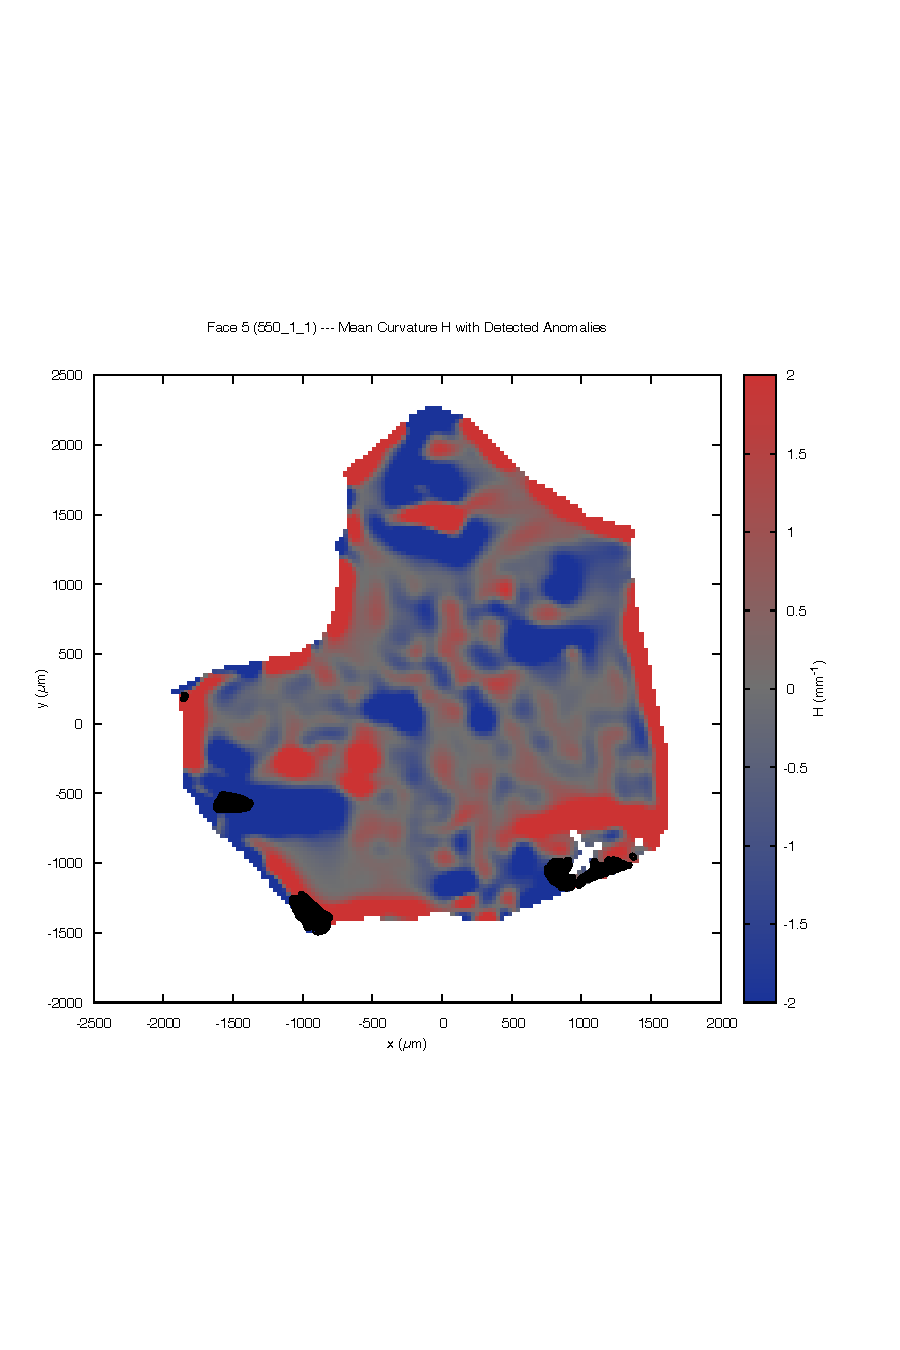
\includegraphics[width=\textwidth]{figures/face5_curvature_anomalies.pdf}
\caption{Mean curvature $H$ (mm$^{-1}$) for Face~5, with anomalies
  (3$\sigma$ residual threshold) marked as black circles.  Gray
  indicates near-zero curvature; red is convex, blue is concave.
  Color palette follows the CIE Luv perceptual uniformity
  recommendations of Nystrom (2008).}
\label{fig:curvature}
\end{figure}

\subsection{Spectral decomposition}

Figure~\ref{fig:spectral} shows the multiresolution decomposition
of the same face into six frequency bands.  The coarsest level
captures the overall shape (a gentle bowl with ${\sim}500$~$\mu$m
peak-to-peak).  Successive bands reveal medium-scale undulations
and fine-scale roughness.  The finest band (Band~4) shows features
at the grid resolution (${\sim}5$~$\mu$m), where particle
inclusions and polishing artifacts are most visible.

\begin{figure}[htbp]
\centering
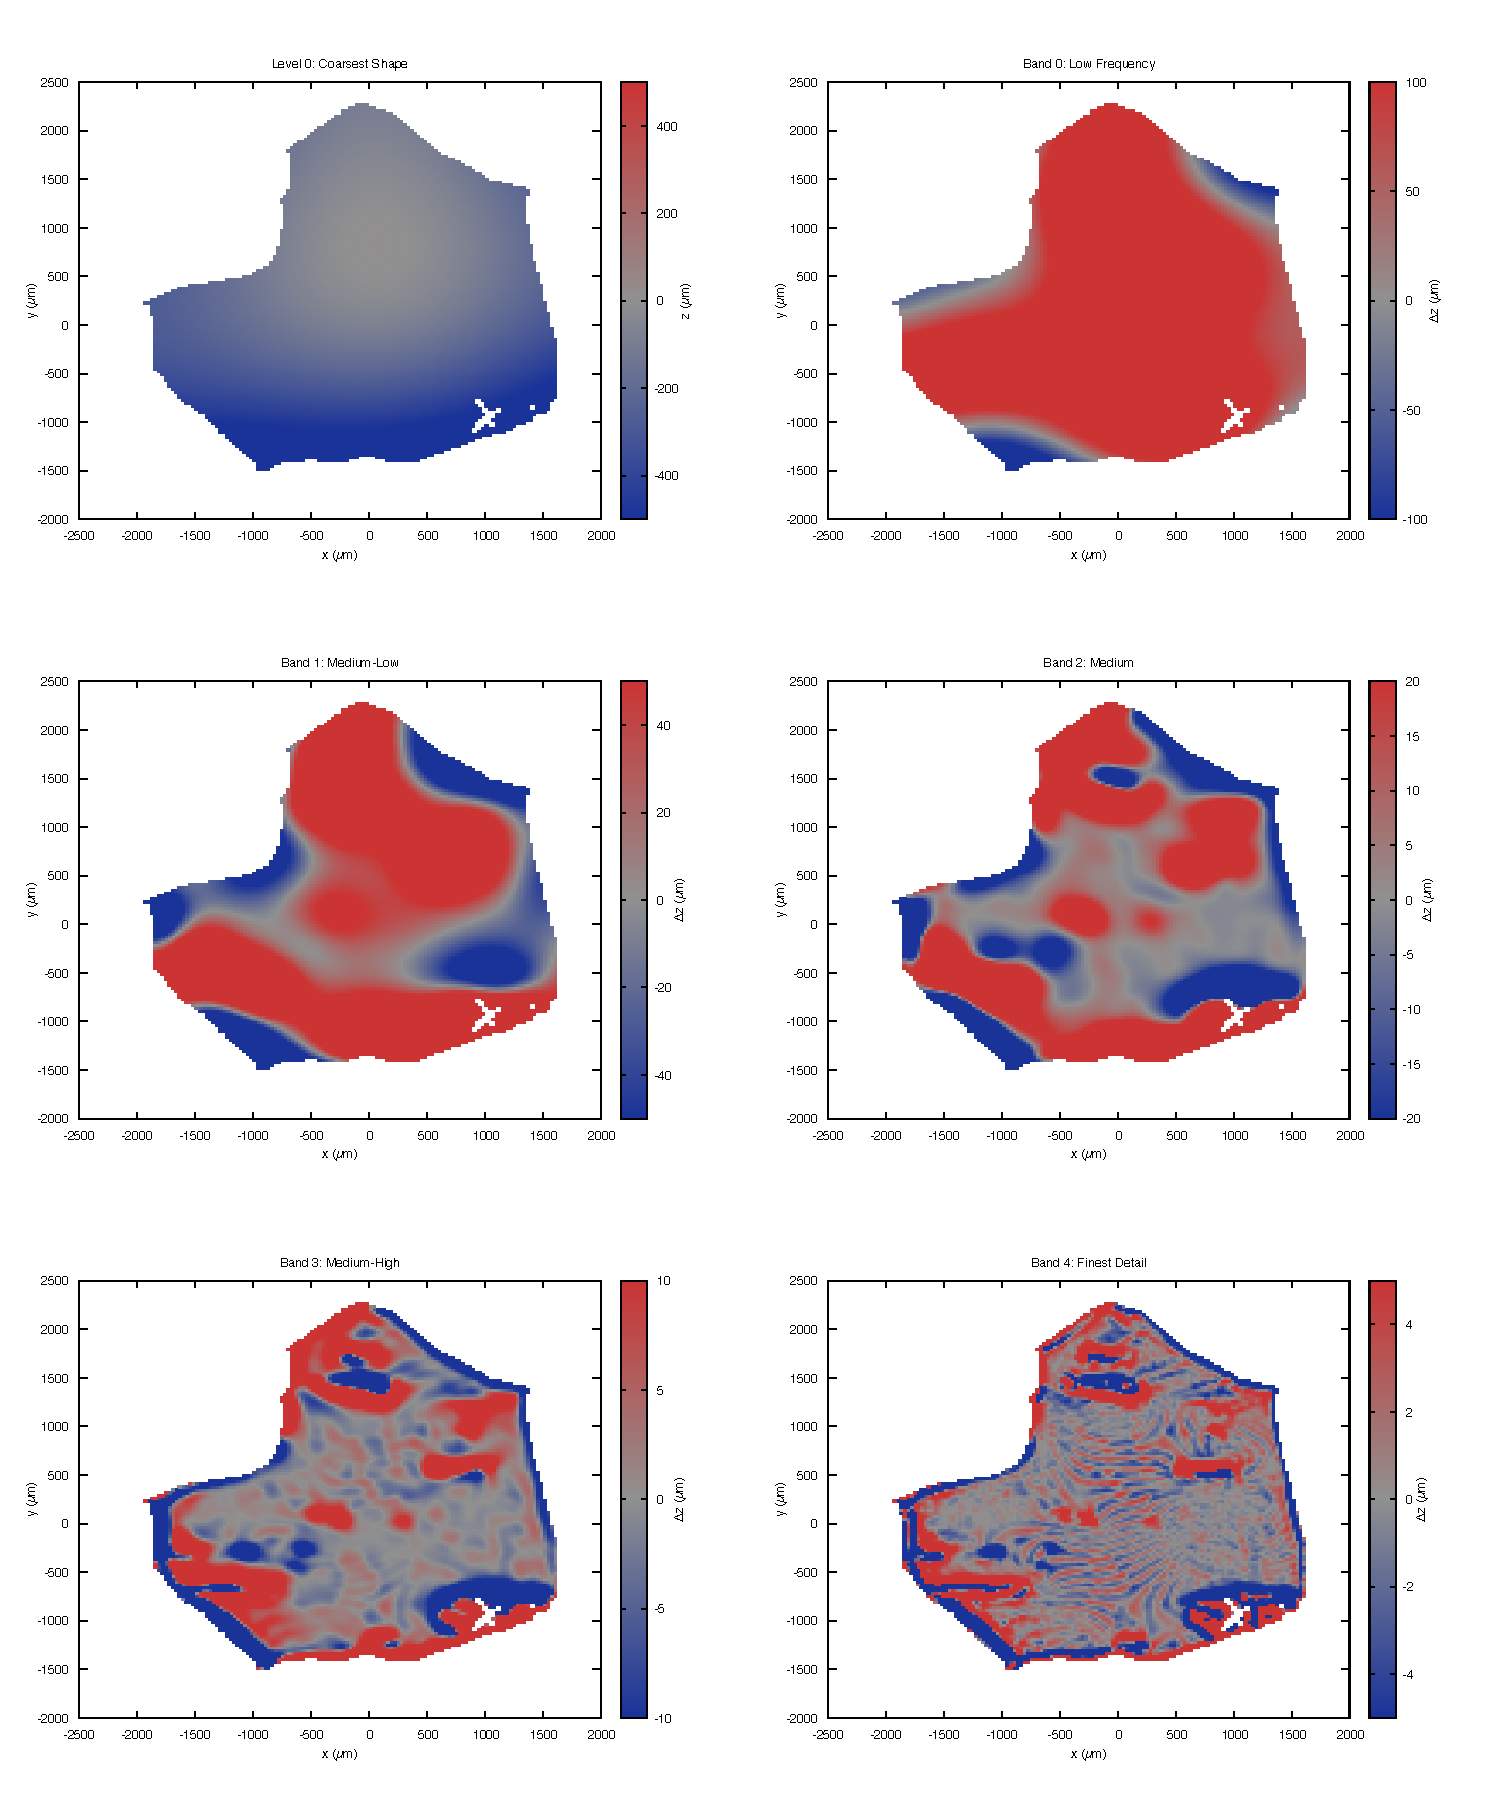
\includegraphics[width=\textwidth]{figures/face5_spectral.pdf}
\caption{Multiresolution height field decomposition of Face~5.
  Top-left: coarsest smoothed level (Gaussian $\sigma = 8$ cells).
  Remaining panels: band-pass differences between successive
  smoothing levels, from low frequency (Band~0) to the finest
  detail (Band~4).  Color scales decrease by approximately $2\times$
  per band, consistent with a power-law roughness spectrum.  All
  values in $\mu$m.}
\label{fig:spectral}
\end{figure}

\subsection{Height field}

Figure~\ref{fig:height} shows the raw height field for Face~5 after
rotation to the $z$-up frame.  The irregular face boundary is
preserved through masking; cells outside the face are omitted.

\begin{figure}[htbp]
\centering
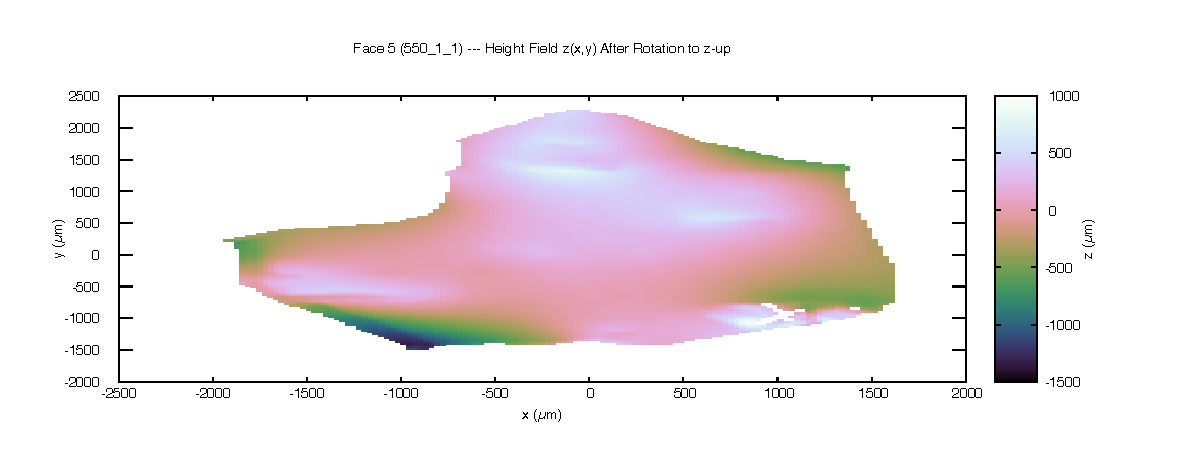
\includegraphics[width=\textwidth]{figures/face5_height.pdf}
\caption{Height field $z(x,y)$ for Face~5 after best-fit plane
  subtraction and rotation.  Units: $\mu$m.  The irregular grain
  face boundary is visible.}
\label{fig:height}
\end{figure}

%% -------------------------------------------------------------------
\section{Curvature Atlas}

The following pages present cotangent-Laplacian mean curvature maps
for all 38 grain faces across four sub-samples.  All plots share a
common color scale of $[-3, +3]$\,mm$^{-1}$, with gray at zero
(flat), red for convex, and blue for concave regions.  Coordinates
are in micrometers.

\begin{figure}[p]
\centering
\textbf{\large Sample 550-1-1}\\[6pt]
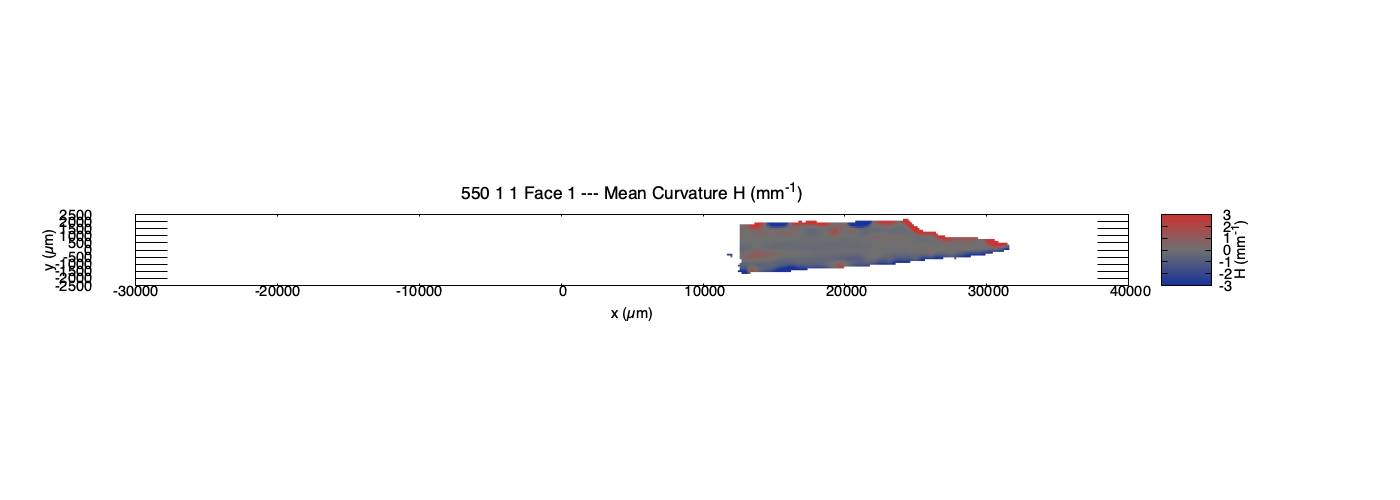
\includegraphics[width=0.48\textwidth]{figures/550-1-1-Face-1.png}\hfill
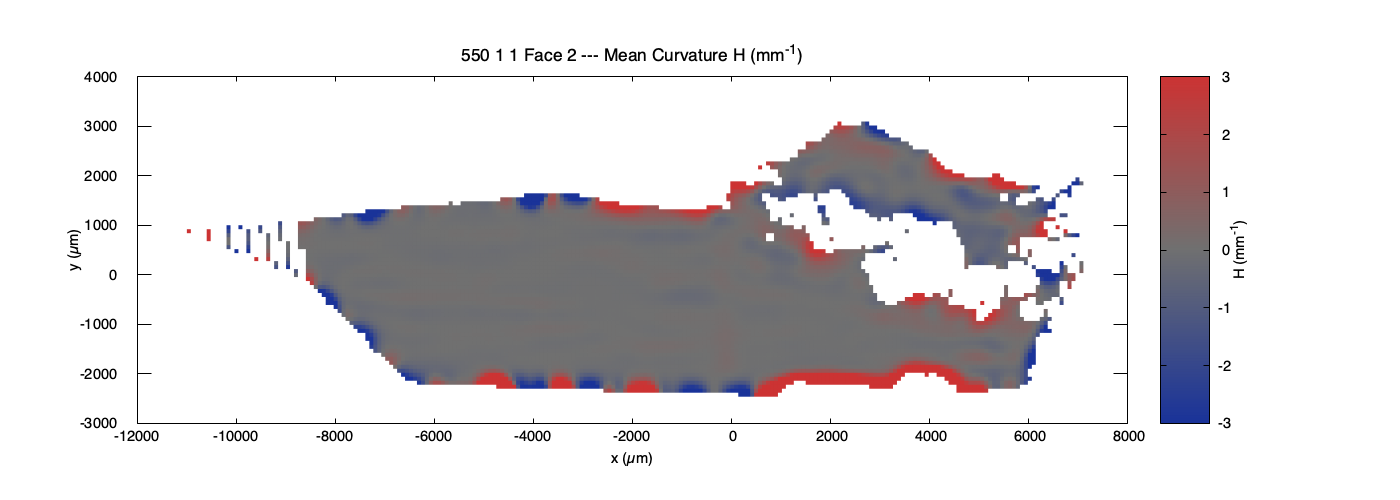
\includegraphics[width=0.48\textwidth]{figures/550-1-1-Face-2.png}\\[4pt]
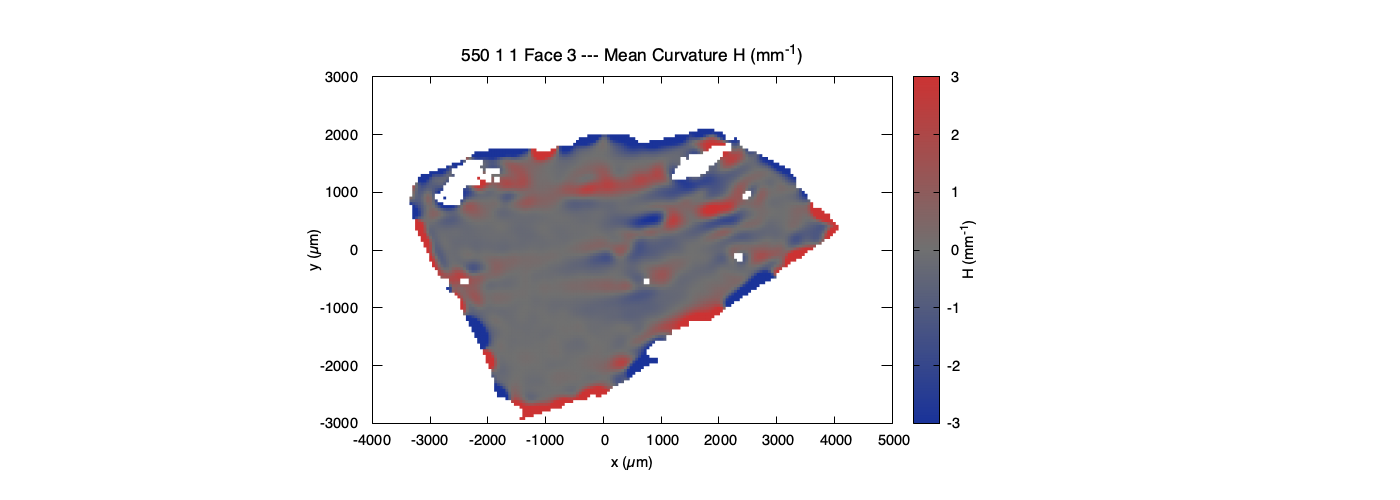
\includegraphics[width=0.48\textwidth]{figures/550-1-1-Face-3.png}\hfill
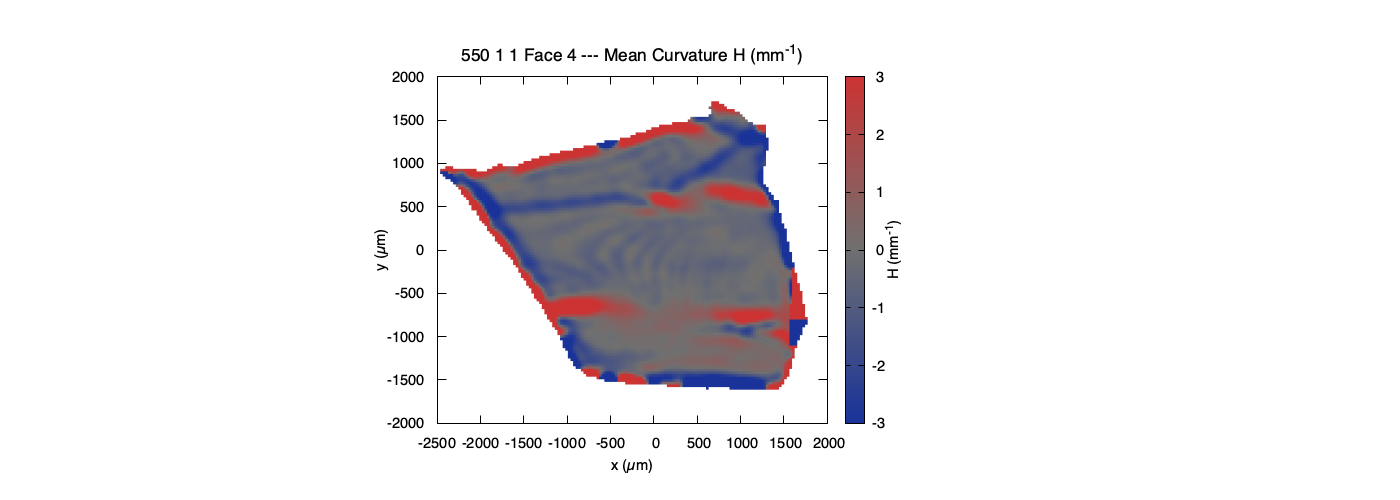
\includegraphics[width=0.48\textwidth]{figures/550-1-1-Face-4.png}\\[4pt]
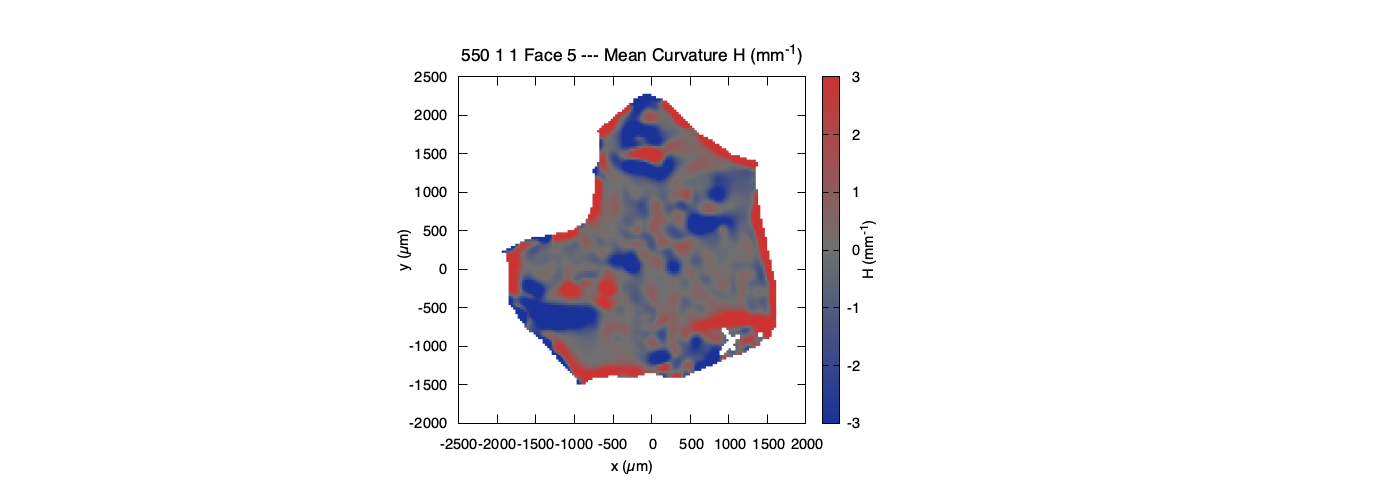
\includegraphics[width=0.48\textwidth]{figures/550-1-1-Face-5.png}\hfill
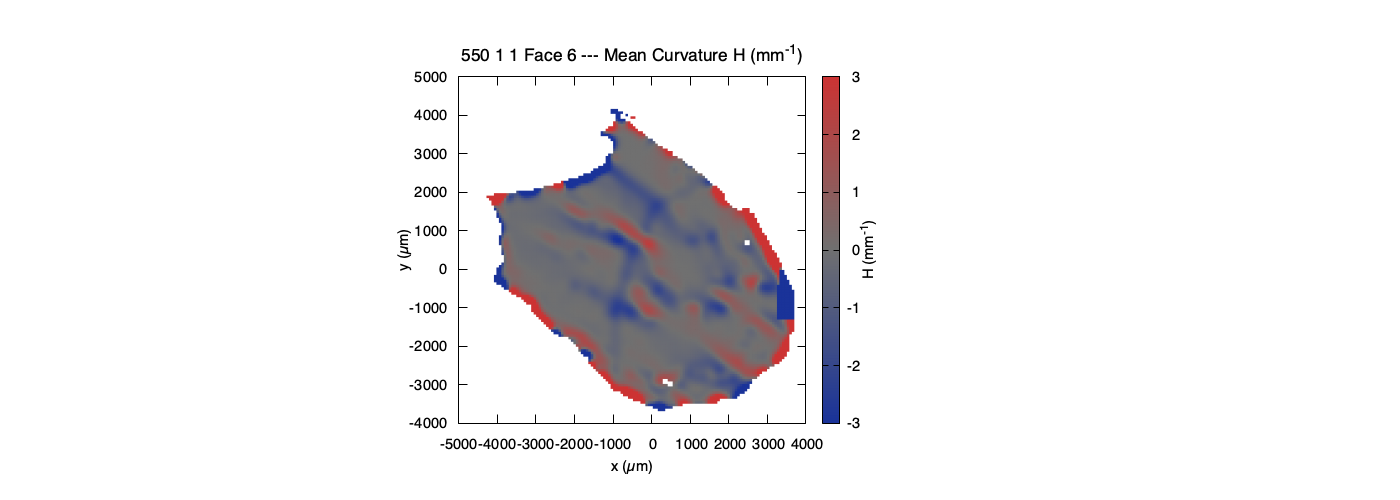
\includegraphics[width=0.48\textwidth]{figures/550-1-1-Face-6.png}\\[4pt]
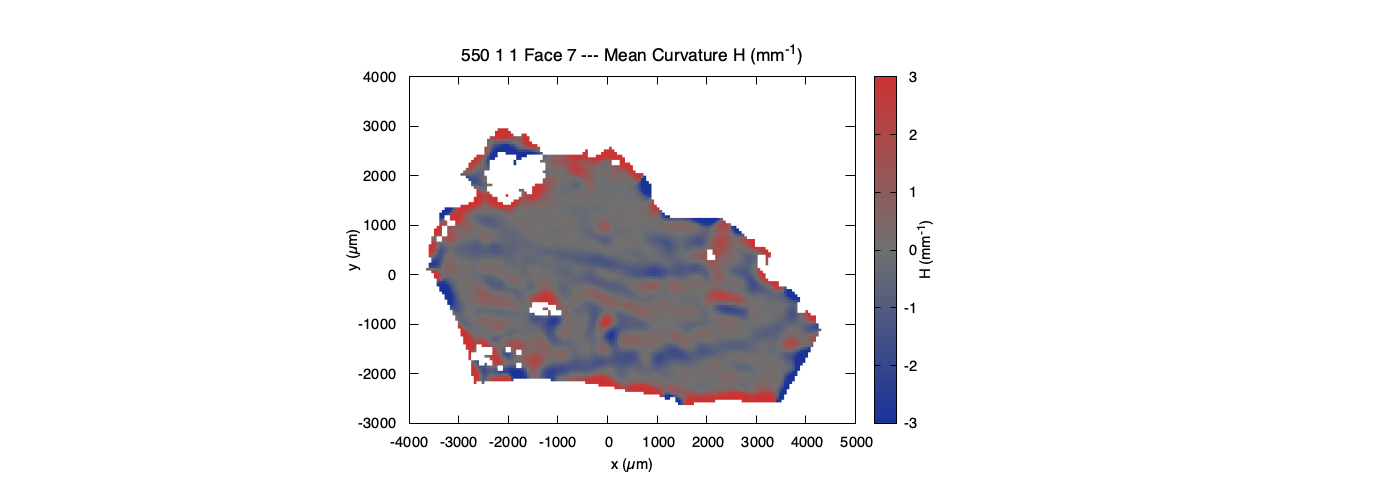
\includegraphics[width=0.48\textwidth]{figures/550-1-1-Face-7.png}\hfill
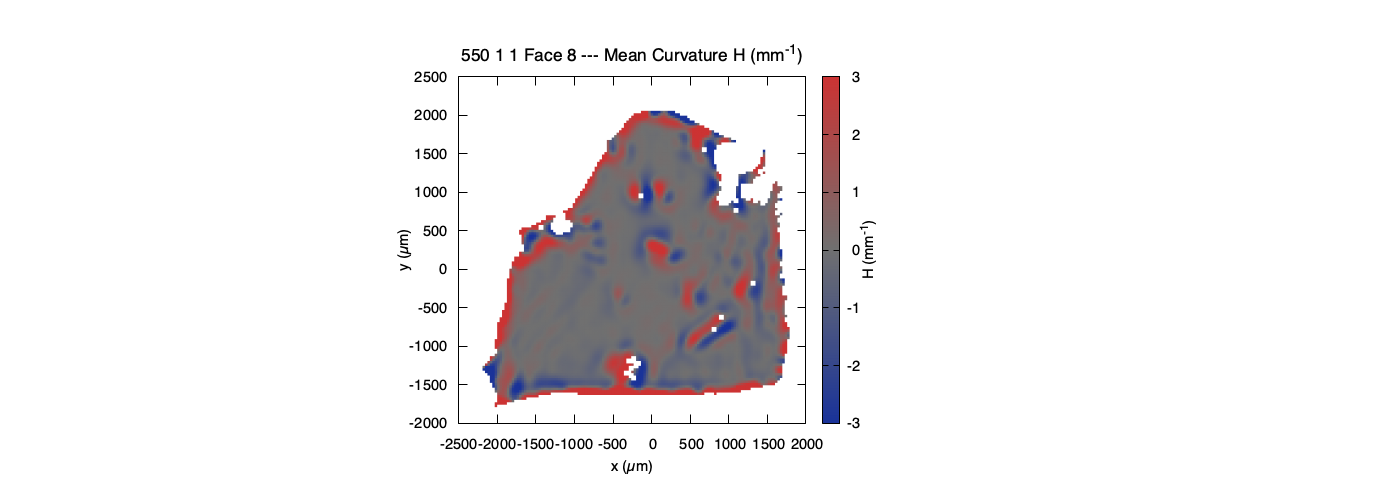
\includegraphics[width=0.48\textwidth]{figures/550-1-1-Face-8.png}
\caption{Mean curvature atlas for sample 550\_1\_1 (8~faces).}
\end{figure}

\begin{figure}[p]
\centering
\textbf{\large Sample 550-1-2}\\[6pt]
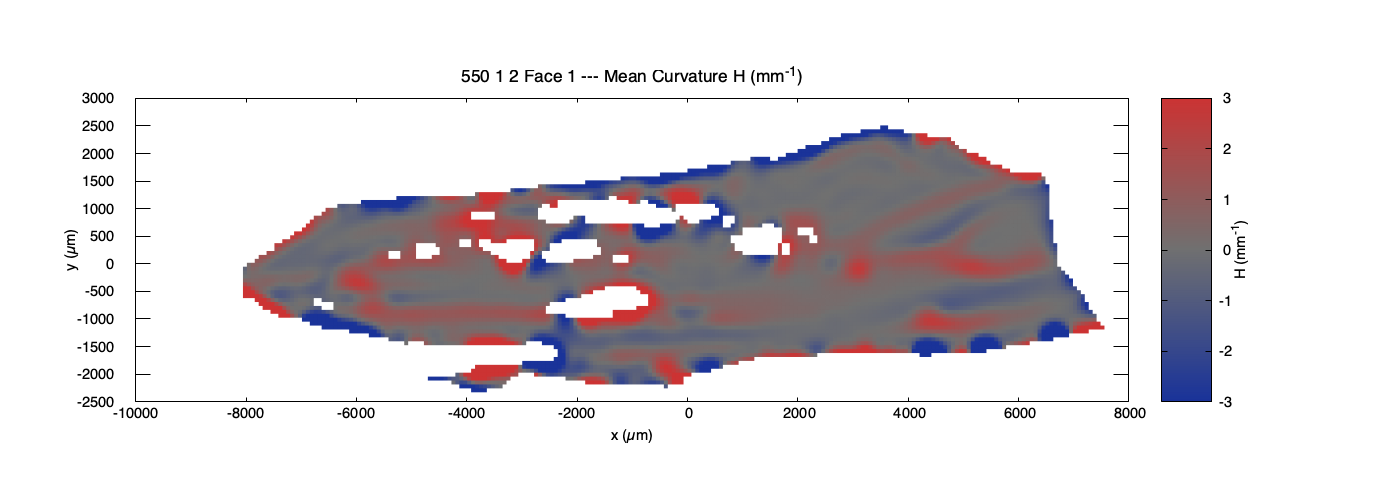
\includegraphics[width=0.48\textwidth]{figures/550-1-2-Face-1.png}\hfill
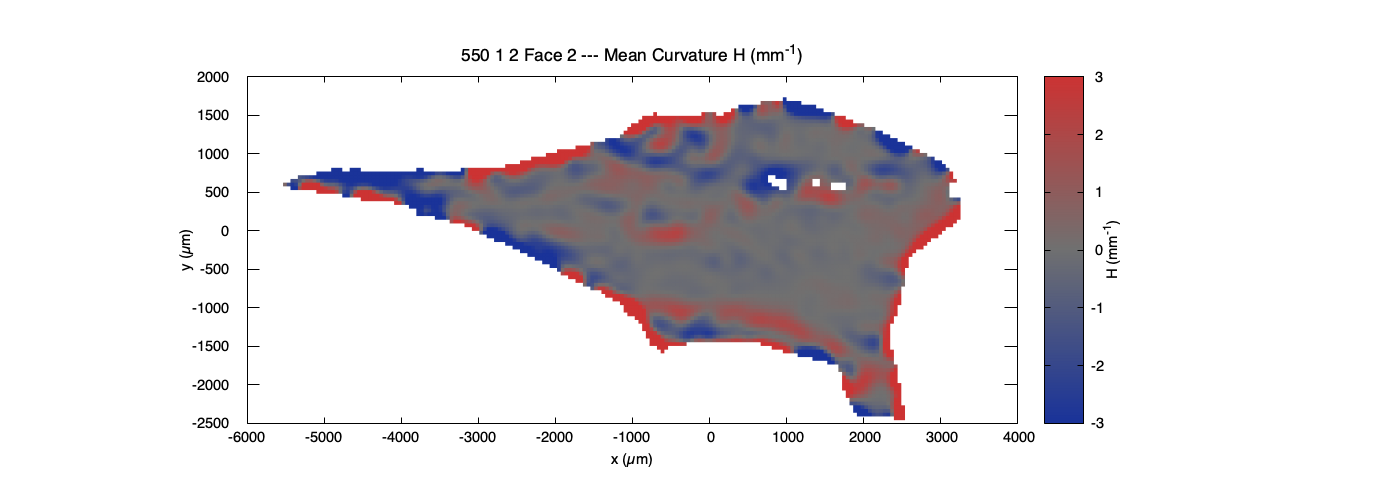
\includegraphics[width=0.48\textwidth]{figures/550-1-2-Face-2.png}\\[4pt]
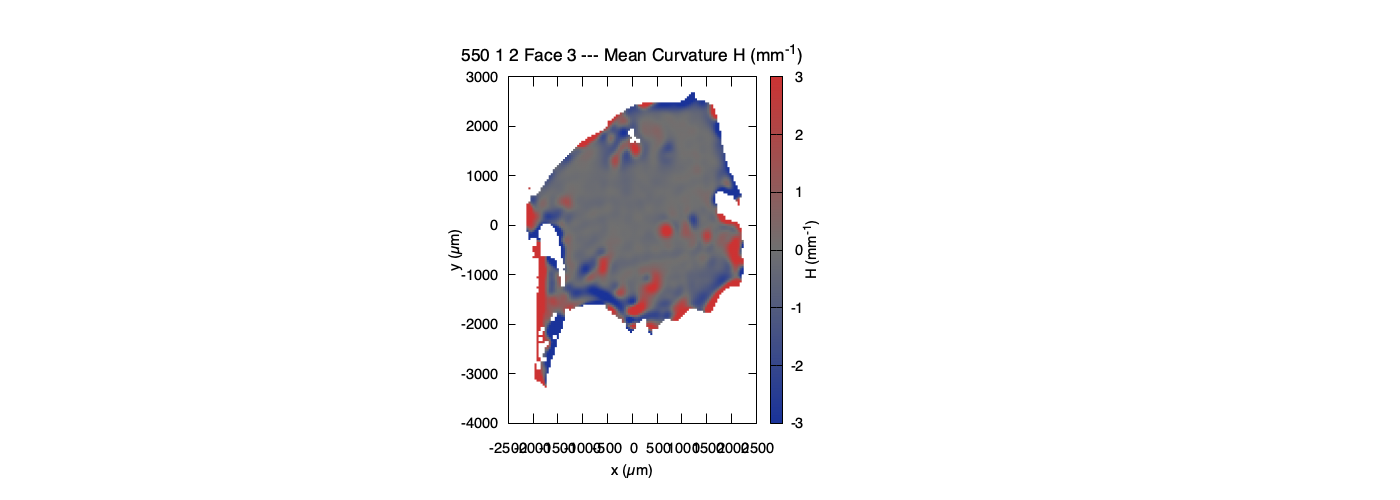
\includegraphics[width=0.48\textwidth]{figures/550-1-2-Face-3.png}\hfill
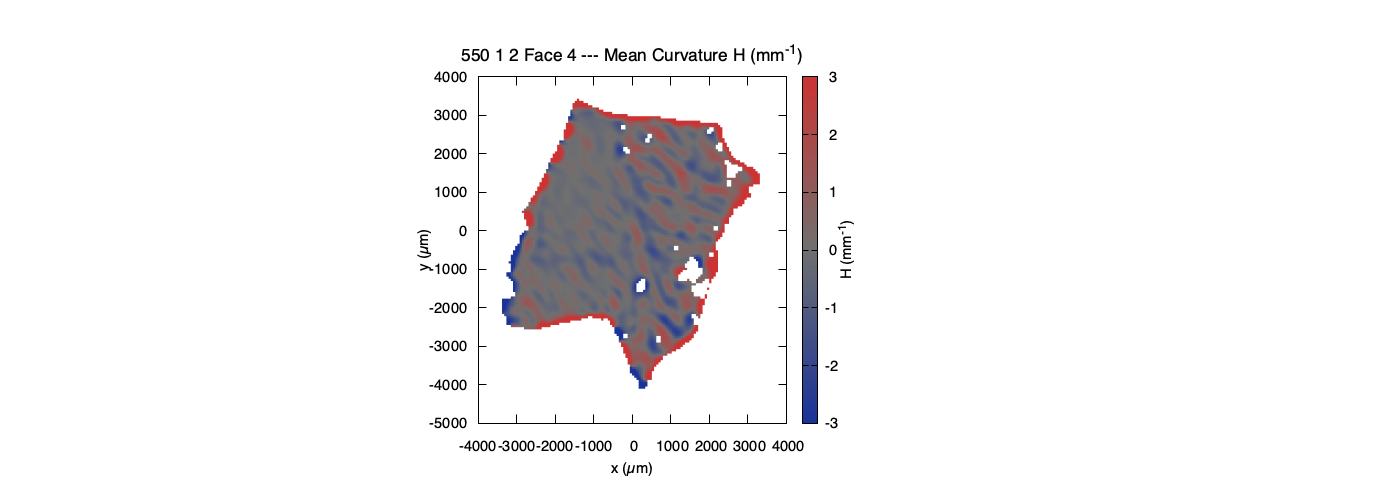
\includegraphics[width=0.48\textwidth]{figures/550-1-2-Face-4.png}\\[4pt]
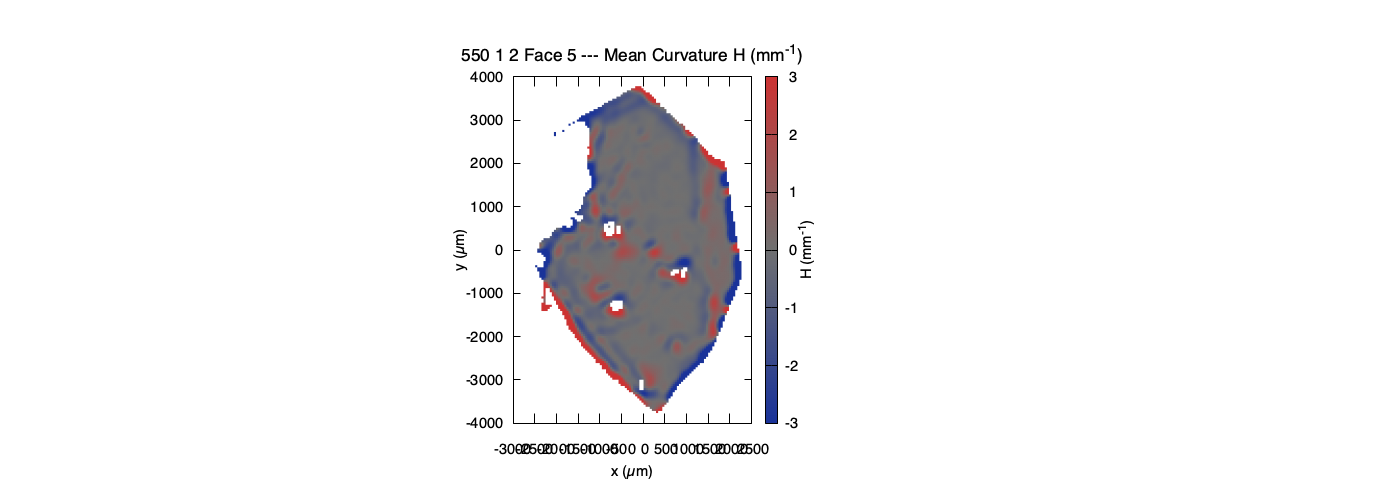
\includegraphics[width=0.48\textwidth]{figures/550-1-2-Face-5.png}\hfill
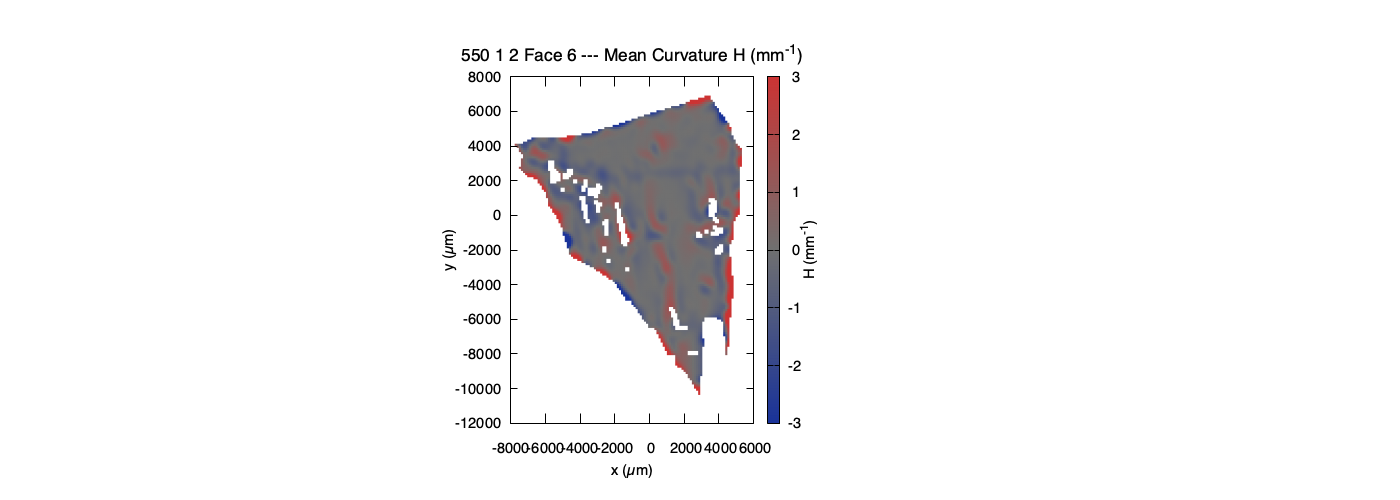
\includegraphics[width=0.48\textwidth]{figures/550-1-2-Face-6.png}\\[4pt]
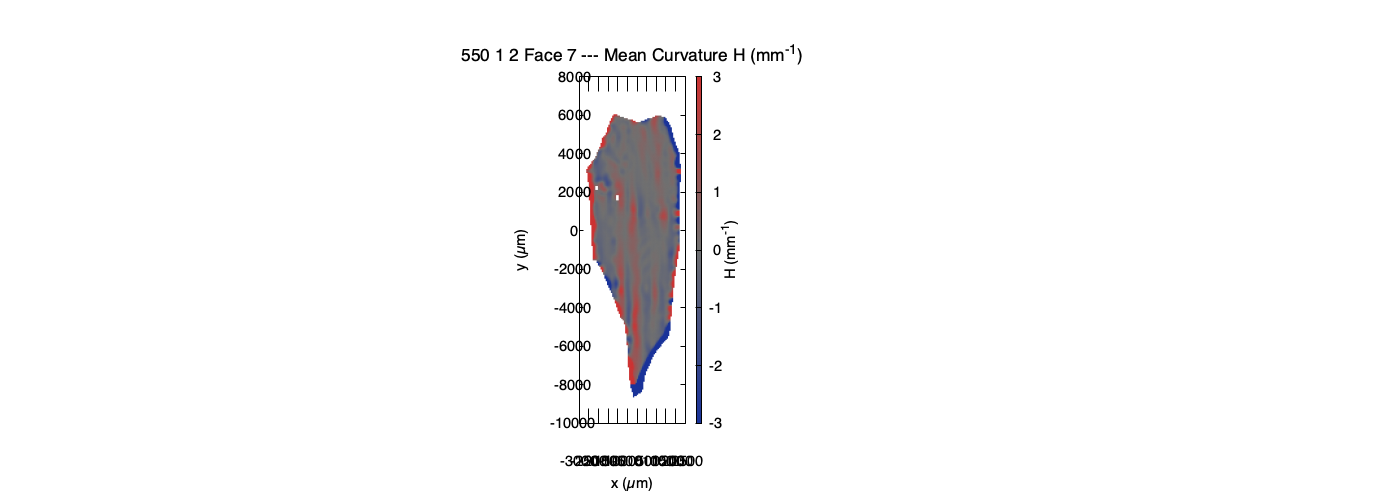
\includegraphics[width=0.48\textwidth]{figures/550-1-2-Face-7.png}\hfill
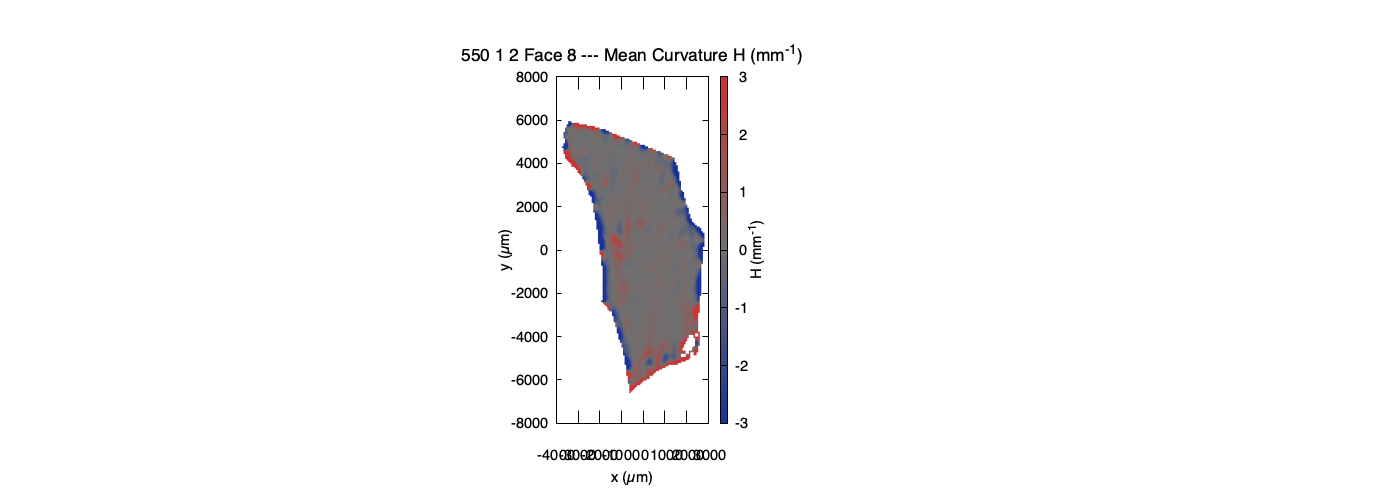
\includegraphics[width=0.48\textwidth]{figures/550-1-2-Face-8.png}
\caption{Mean curvature atlas for sample 550\_1\_2 (faces 1--8 of 12).}
\end{figure}

\begin{figure}[p]
\centering
\textbf{\large Sample 550-1-2 (continued)}\\[6pt]
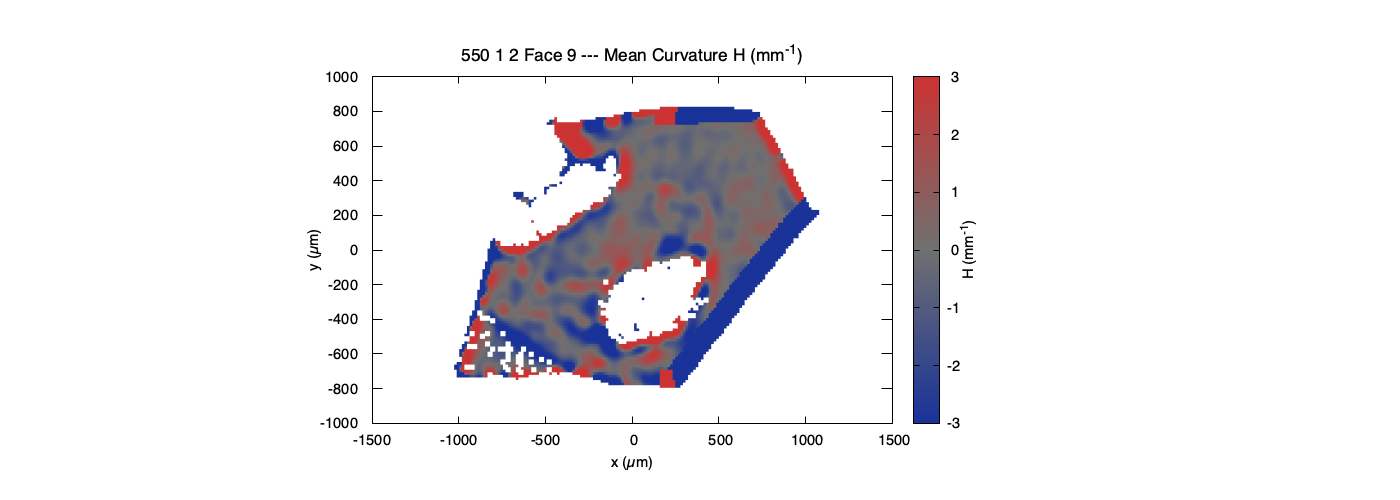
\includegraphics[width=0.48\textwidth]{figures/550-1-2-Face-9.png}\hfill
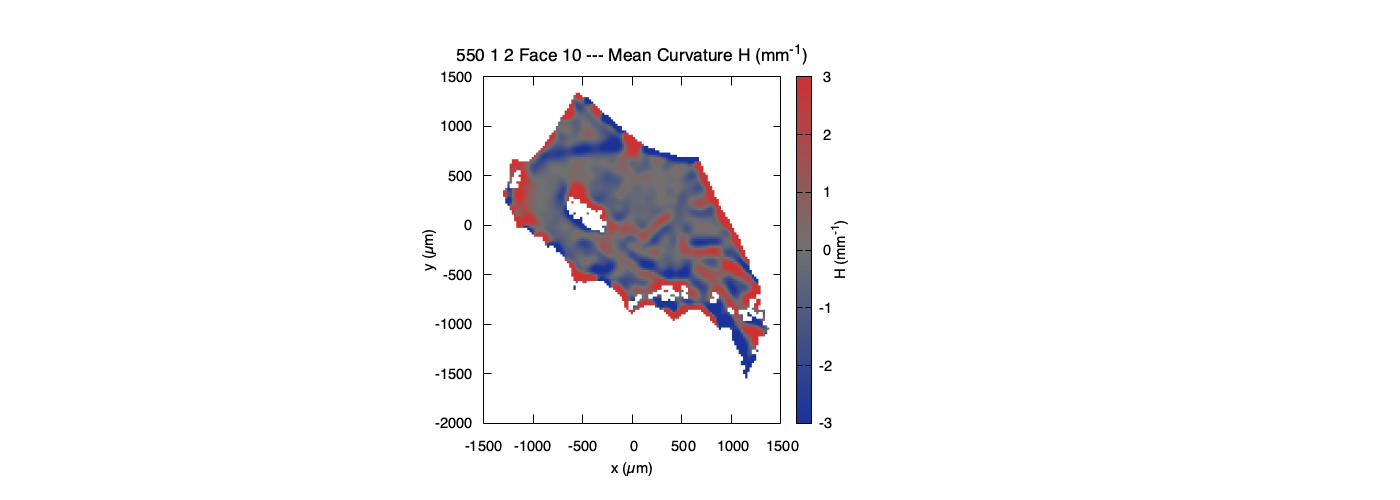
\includegraphics[width=0.48\textwidth]{figures/550-1-2-Face-10.png}\\[4pt]
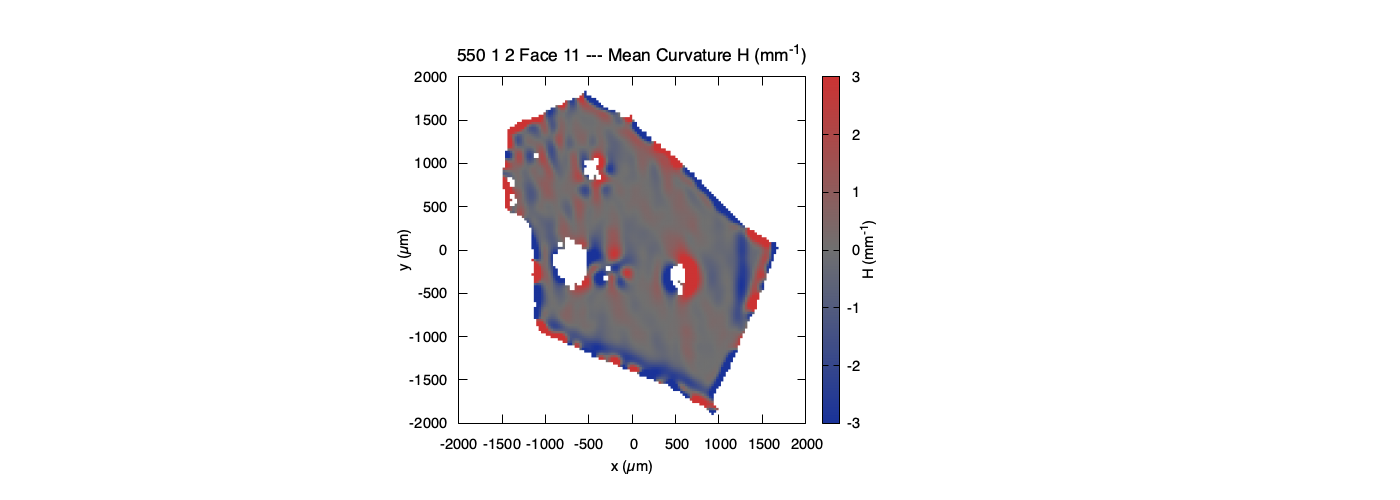
\includegraphics[width=0.48\textwidth]{figures/550-1-2-Face-11.png}\hfill
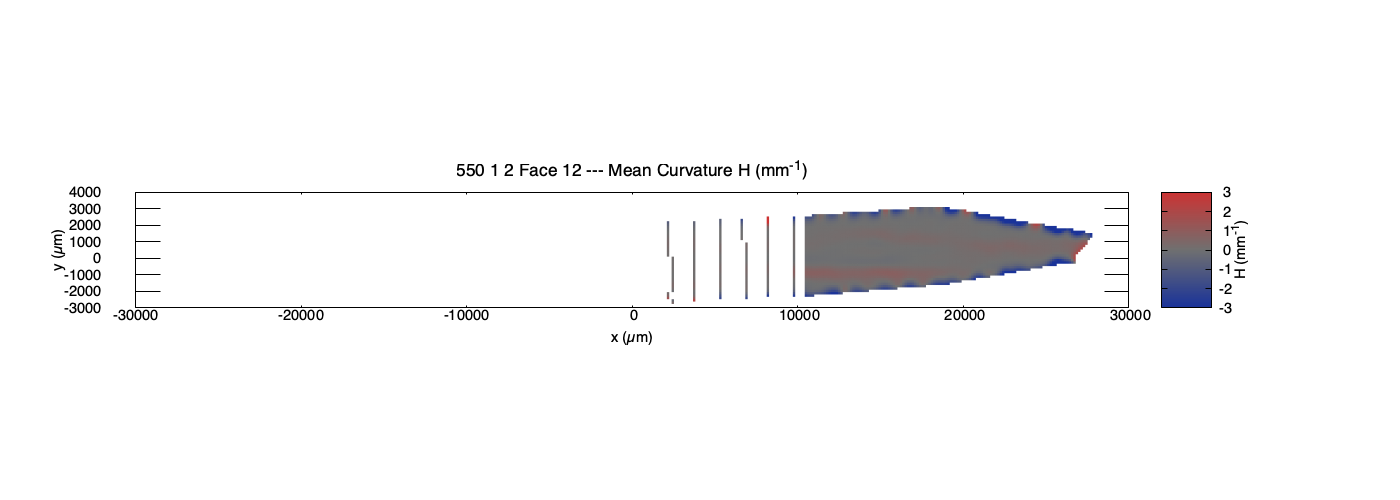
\includegraphics[width=0.48\textwidth]{figures/550-1-2-Face-12.png}
\caption{Mean curvature atlas for sample 550\_1\_2 (faces 9--12 of 12).}
\end{figure}

\begin{figure}[p]
\centering
\textbf{\large Sample 550-1-3}\\[6pt]
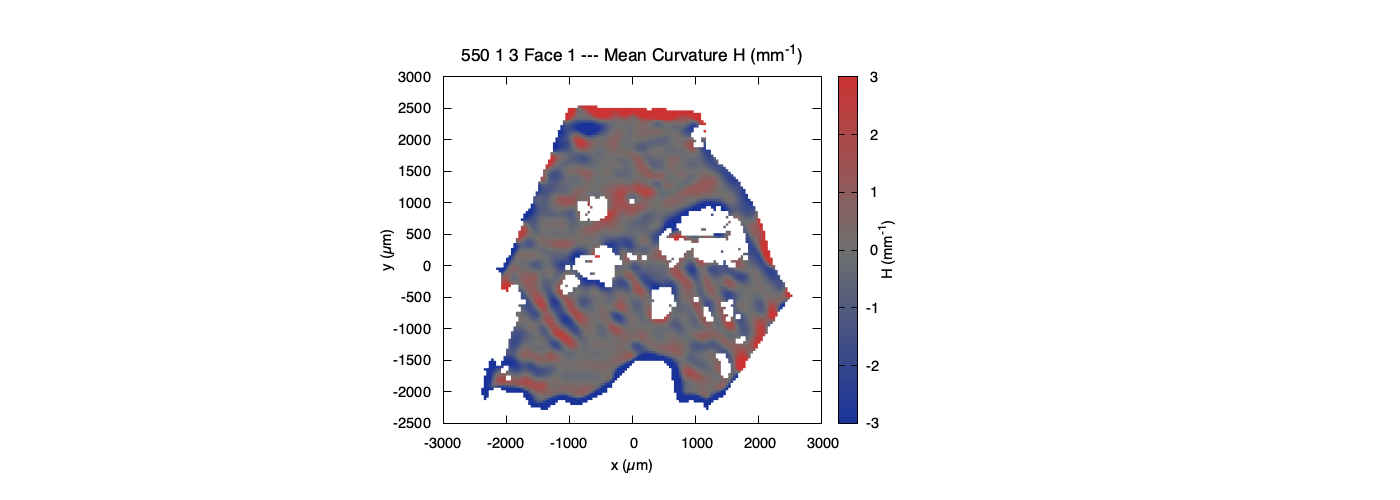
\includegraphics[width=0.48\textwidth]{figures/550-1-3-Face-1.png}\hfill
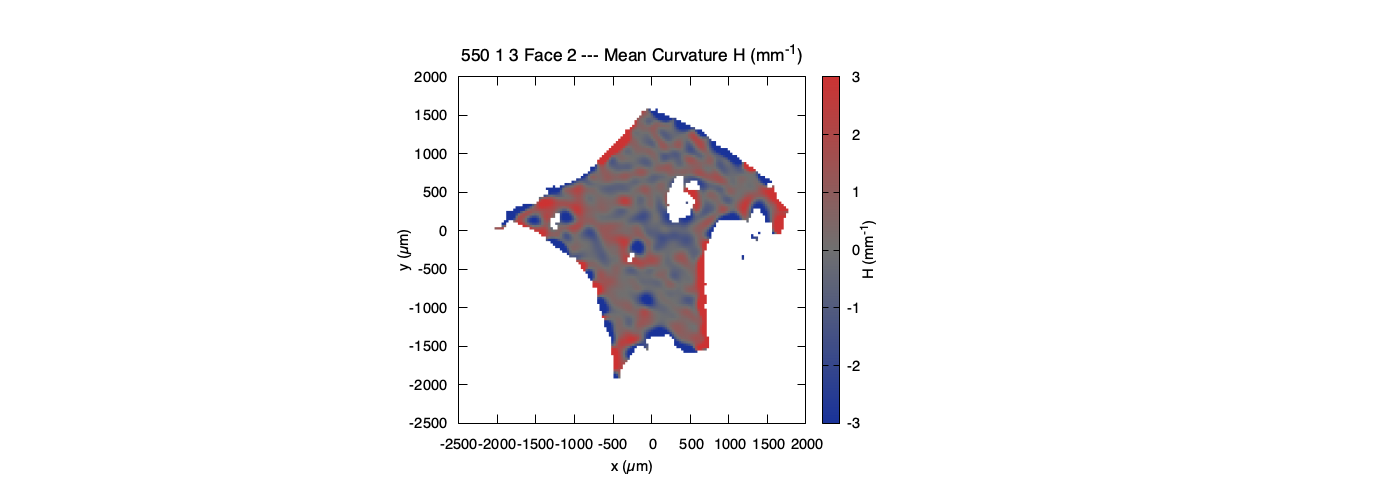
\includegraphics[width=0.48\textwidth]{figures/550-1-3-Face-2.png}\\[4pt]
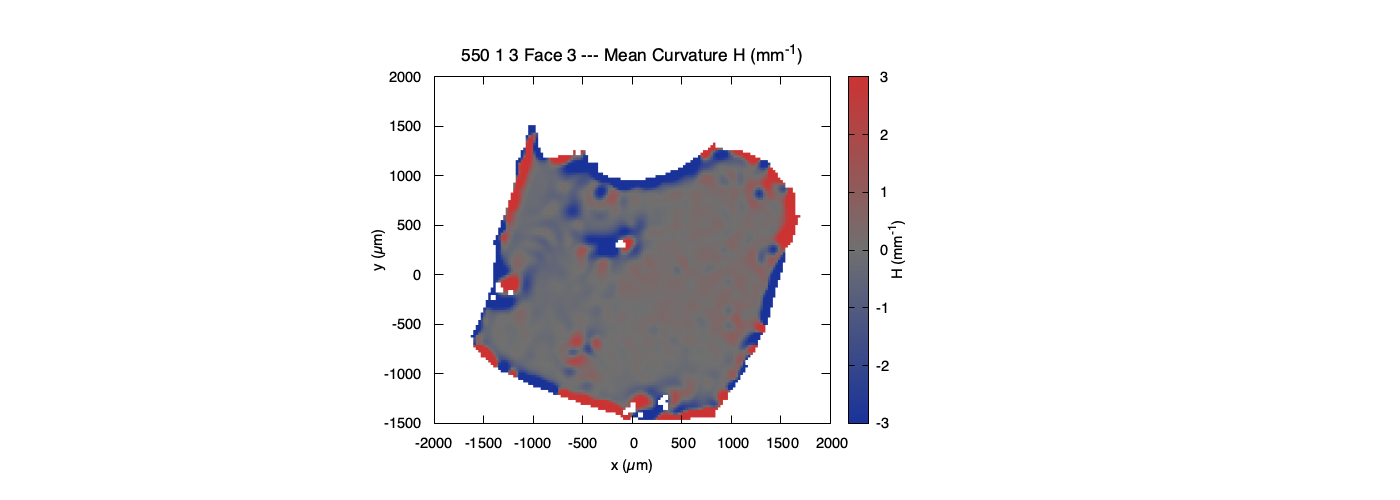
\includegraphics[width=0.48\textwidth]{figures/550-1-3-Face-3.png}\hfill
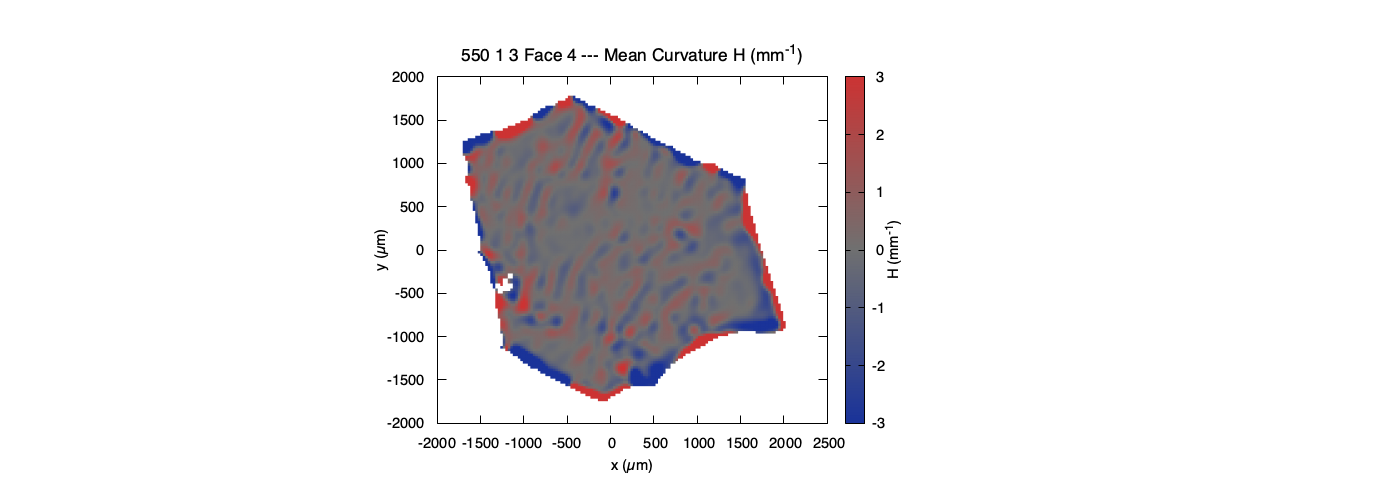
\includegraphics[width=0.48\textwidth]{figures/550-1-3-Face-4.png}\\[4pt]
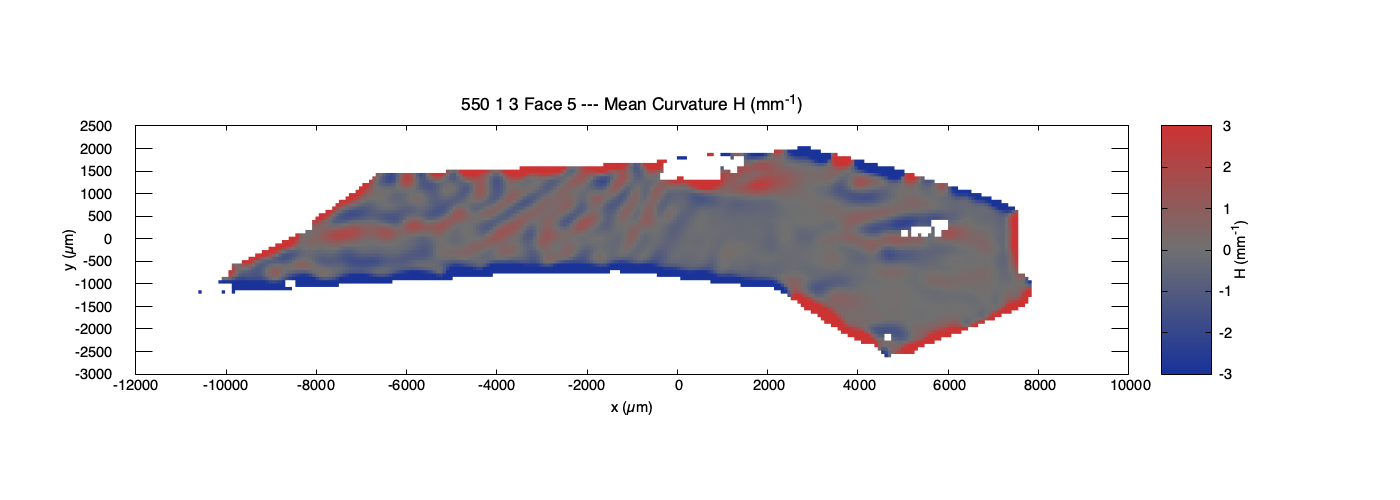
\includegraphics[width=0.48\textwidth]{figures/550-1-3-Face-5.png}\hfill
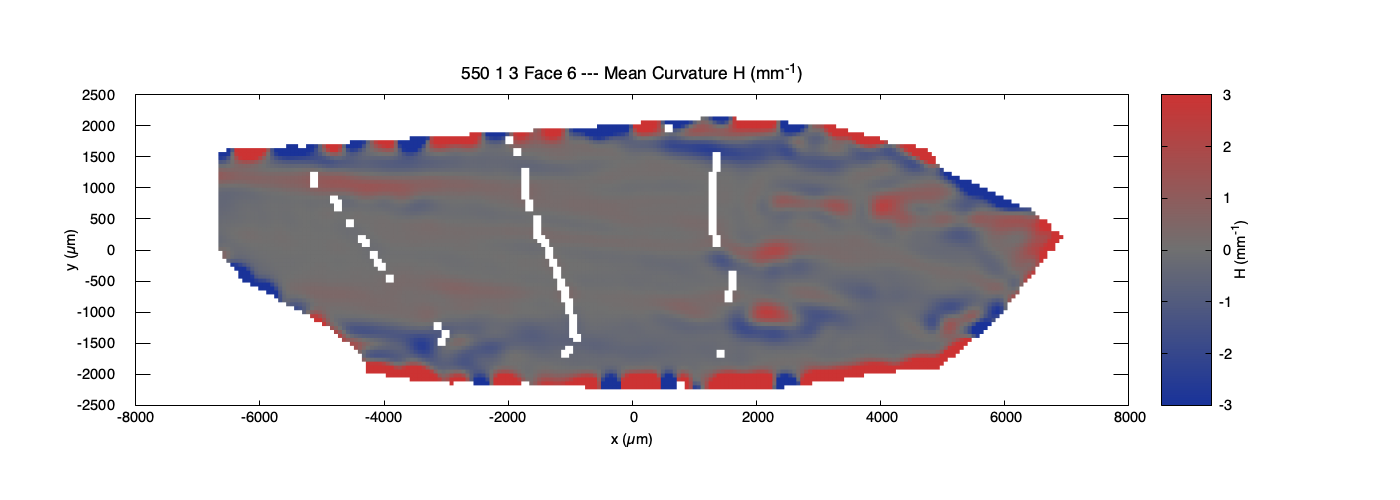
\includegraphics[width=0.48\textwidth]{figures/550-1-3-Face-6.png}\\[4pt]
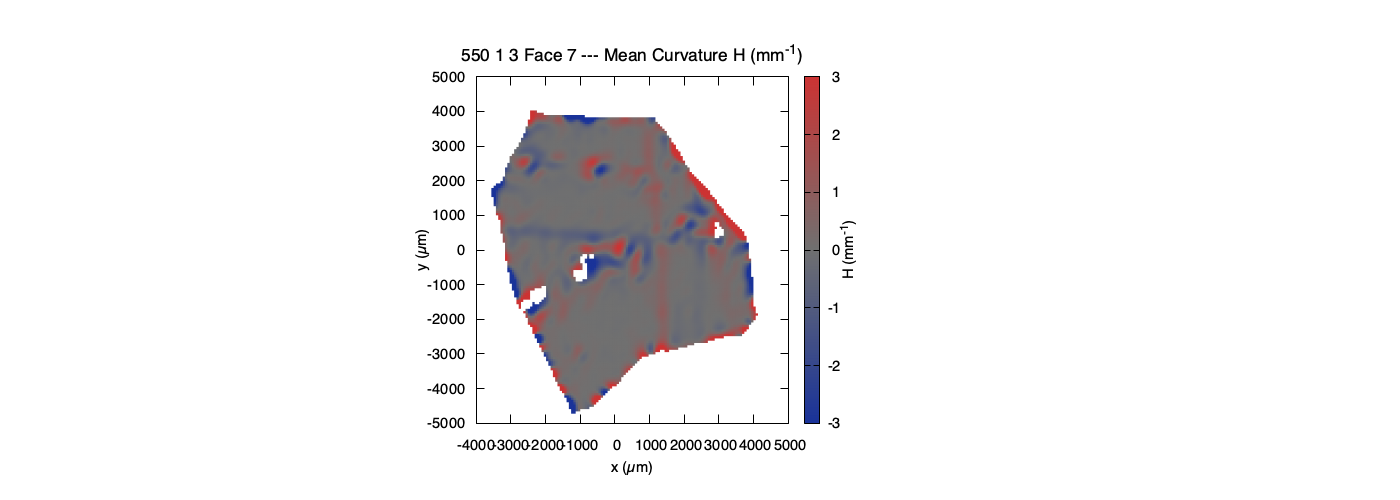
\includegraphics[width=0.48\textwidth]{figures/550-1-3-Face-7.png}\hfill
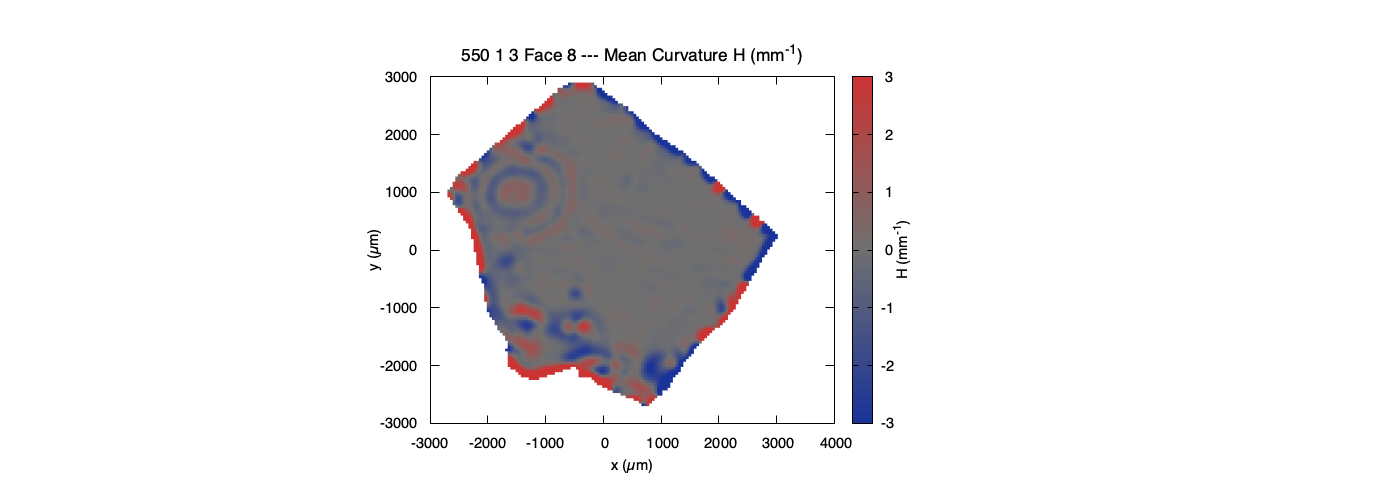
\includegraphics[width=0.48\textwidth]{figures/550-1-3-Face-8.png}\\[4pt]
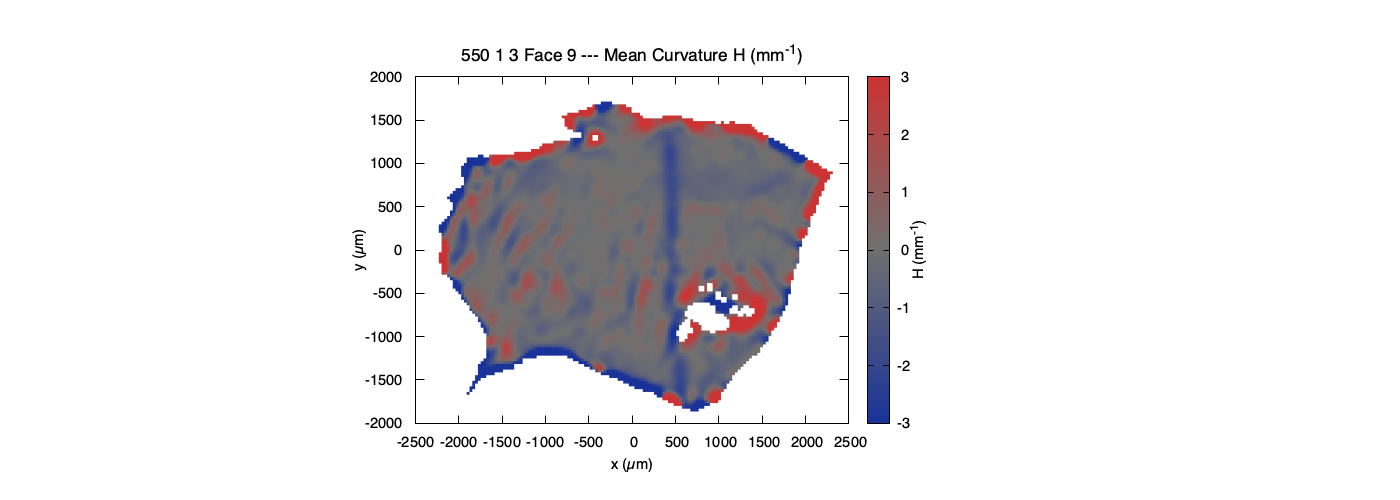
\includegraphics[width=0.48\textwidth]{figures/550-1-3-Face-9.png}
\caption{Mean curvature atlas for sample 550\_1\_3 (9~faces).}
\end{figure}

\begin{figure}[p]
\centering
\textbf{\large Sample 550-1-4}\\[6pt]
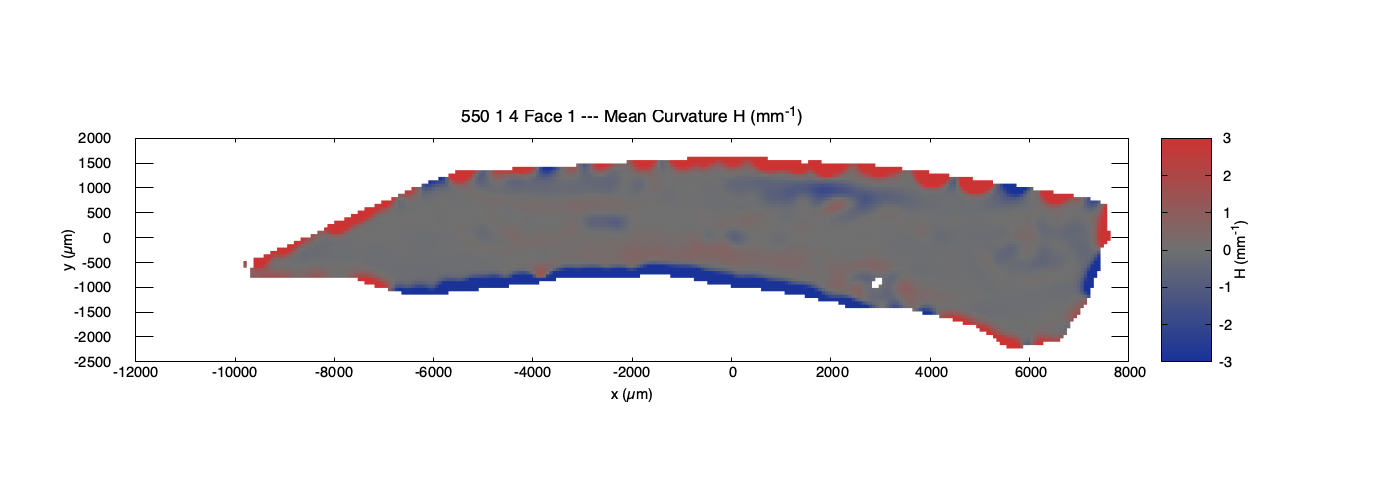
\includegraphics[width=0.48\textwidth]{figures/550-1-4-Face-1.png}\hfill
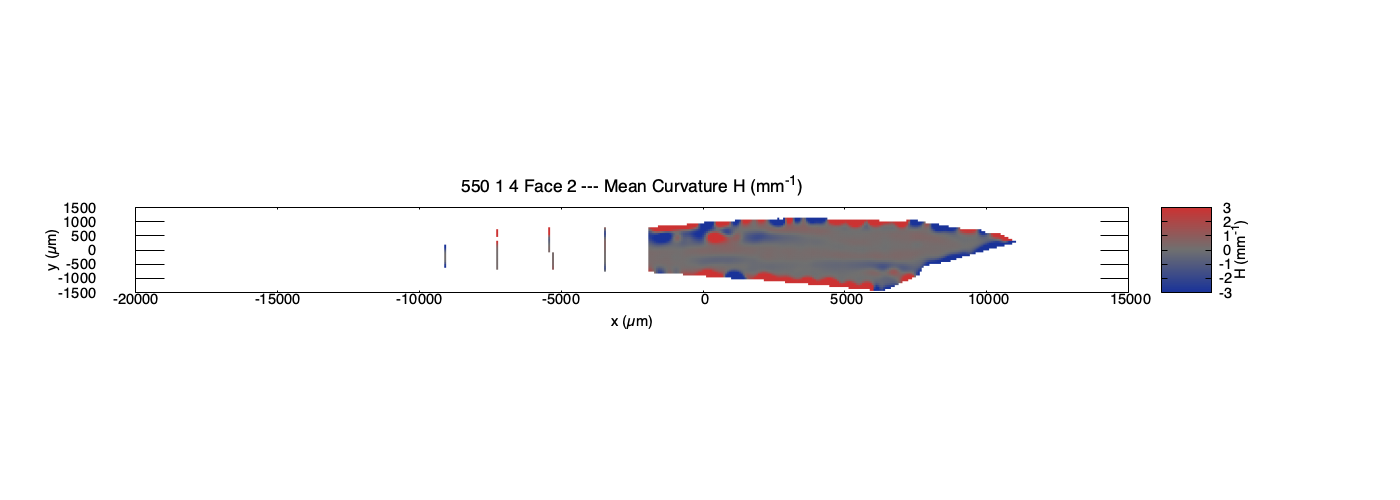
\includegraphics[width=0.48\textwidth]{figures/550-1-4-Face-2.png}\\[4pt]
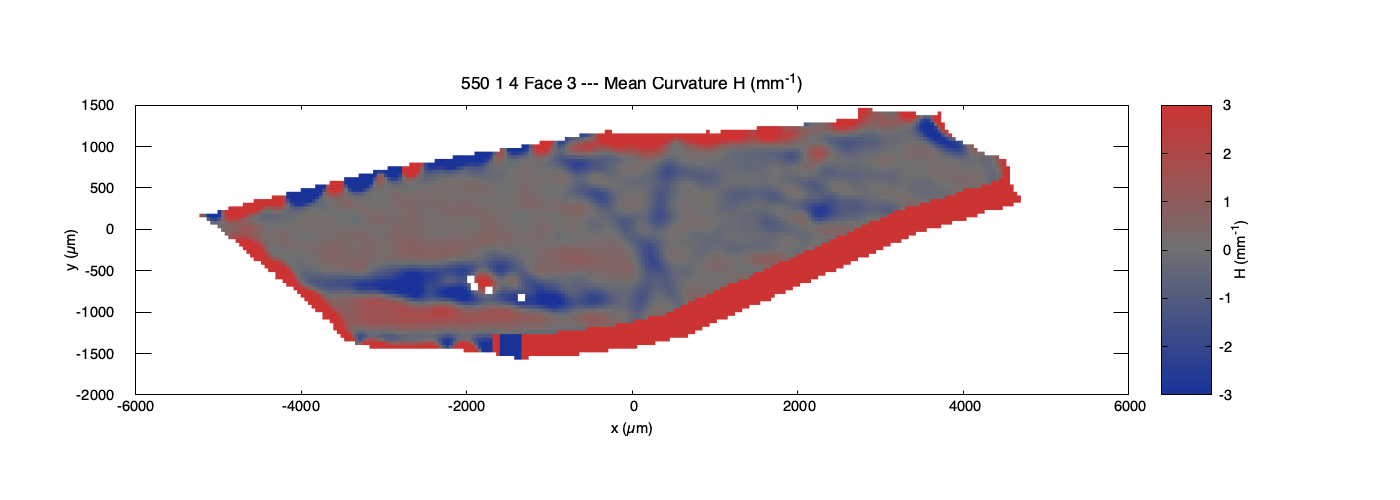
\includegraphics[width=0.48\textwidth]{figures/550-1-4-Face-3.png}\hfill
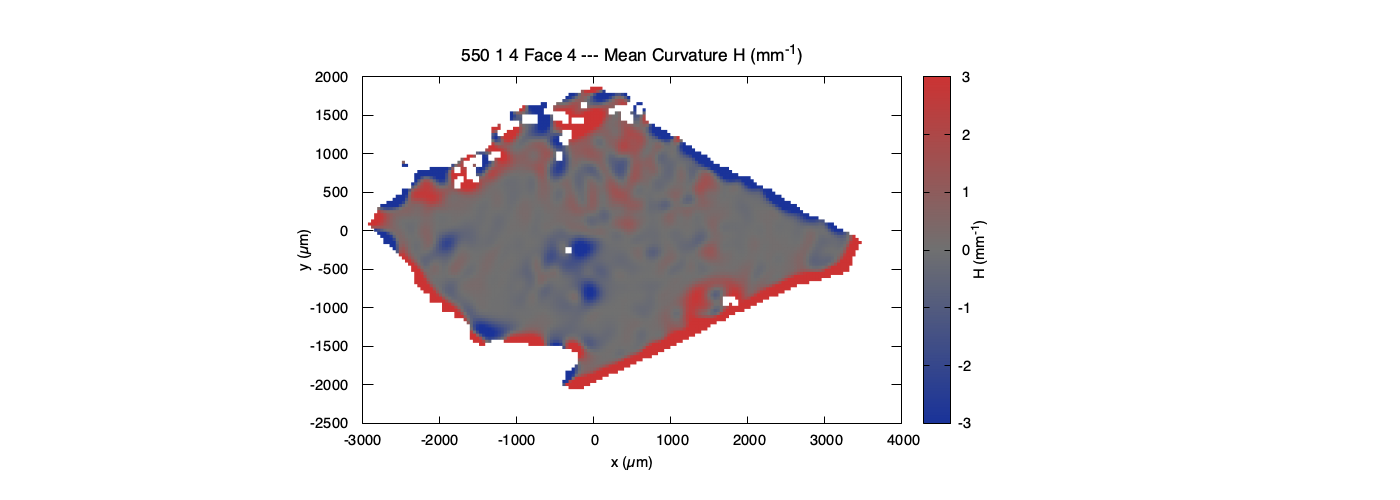
\includegraphics[width=0.48\textwidth]{figures/550-1-4-Face-4.png}\\[4pt]
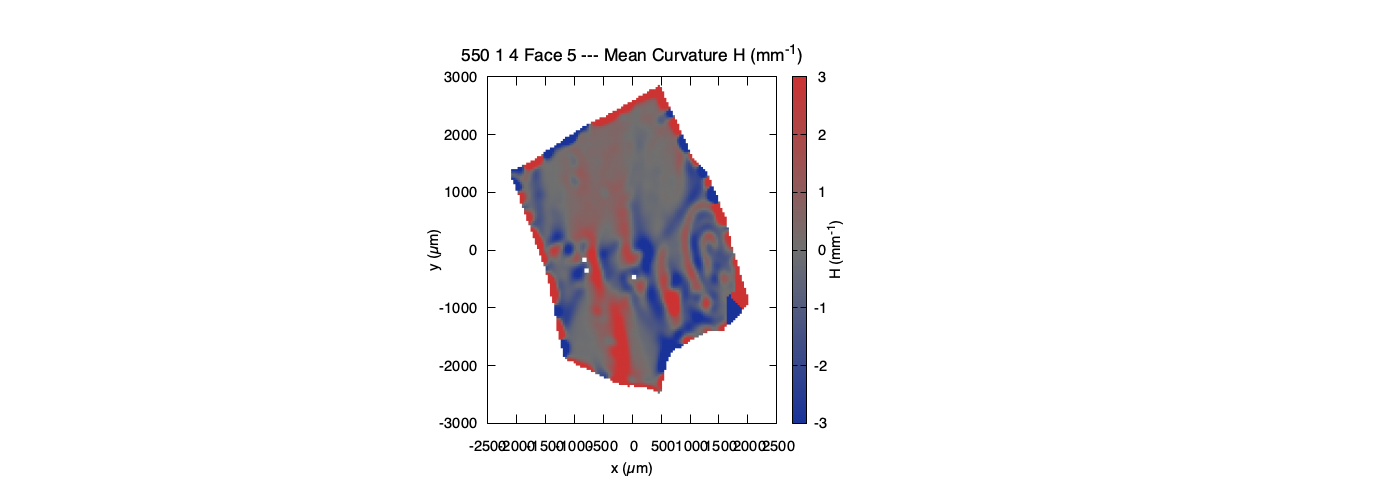
\includegraphics[width=0.48\textwidth]{figures/550-1-4-Face-5.png}\hfill
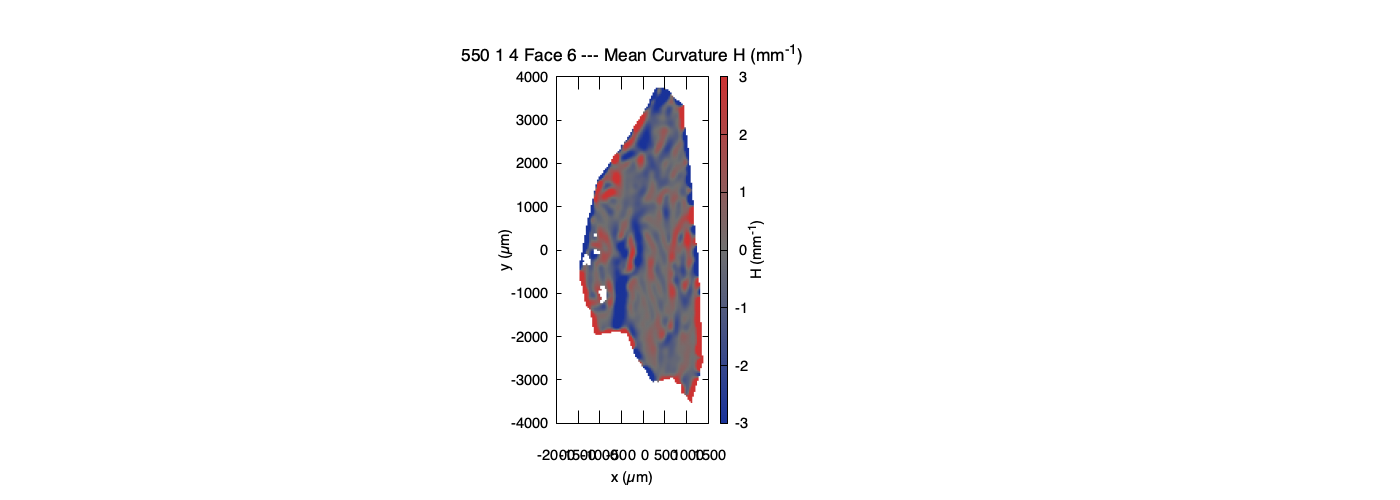
\includegraphics[width=0.48\textwidth]{figures/550-1-4-Face-6.png}\\[4pt]
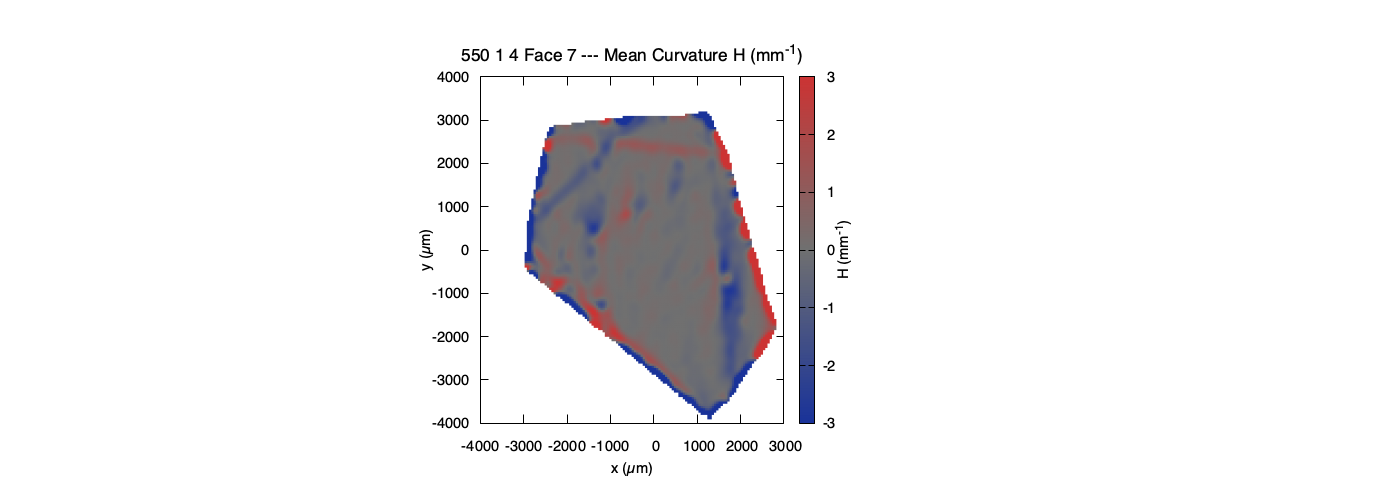
\includegraphics[width=0.48\textwidth]{figures/550-1-4-Face-7.png}\hfill
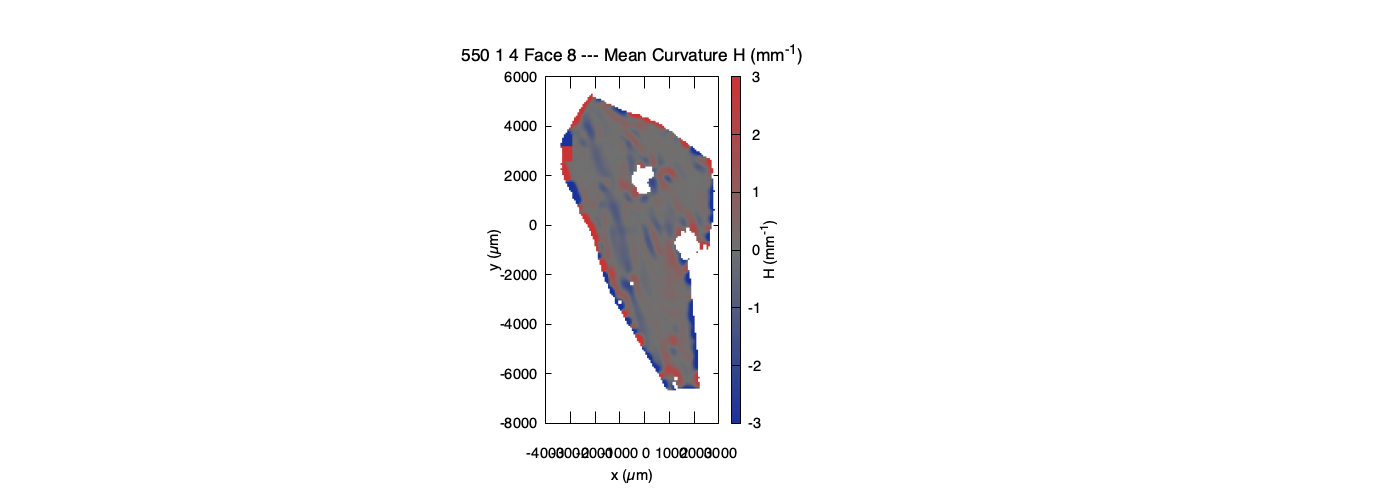
\includegraphics[width=0.48\textwidth]{figures/550-1-4-Face-8.png}\\[4pt]
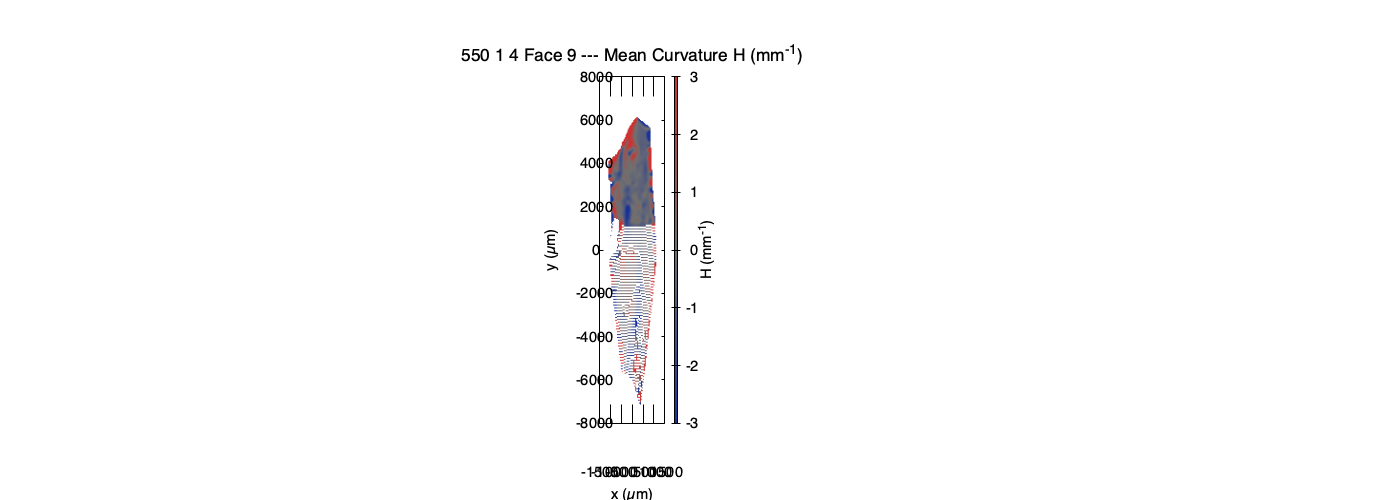
\includegraphics[width=0.48\textwidth]{figures/550-1-4-Face-9.png}
\caption{Mean curvature atlas for sample 550\_1\_4 (9~faces).}
\end{figure}

\clearpage

%% -------------------------------------------------------------------
\section{Usage}

\subsection{Building}

\begin{lstlisting}
cd Al_Ga/plylib/src && cm3 -override
cd Al_Ga/meshlib/src && cm3 -override
cd Al_Ga/facetlib/src && cm3 -override
cd Al_Ga/curvlib/src && cm3 -override
cd Al_Ga/plydemo/src && cm3 -override
\end{lstlisting}

\subsection{Single face analysis}

\begin{lstlisting}
plydemo 550_1_1/Face_1_mesh.ply
\end{lstlisting}

Prints mesh statistics, curvature summary, and detected anomalies
to standard output.

\subsection{Segmentation of a full surface scan}

\begin{lstlisting}
plydemo -segment -angle 10 -minverts 500 -maxtilt 30 \
  AlGa_LEXT_surface_downsample_1024_6.ply
\end{lstlisting}

Segments the surface into planar grain faces, filters by tilt
angle, and reports per-region curvature and anomaly statistics.

\subsection{Multiresolution contour output}

\begin{lstlisting}
mkdir outdir
plydemo -contour outdir -levels 6 550_1_1/Face_5_mesh.ply
gnuplot outdir/face_contours.gp
\end{lstlisting}

Writes gnuplot-compatible grid data files for height levels,
band-pass differences, curvature, residuals, and anomaly points.
All coordinates are output in micrometers; curvature in
mm$^{-1}$.

%% -------------------------------------------------------------------
\section{Color}

The color palette for curvature maps follows the recommendations
of the CIE~Luv perceptual uniformity analysis in the ``Curves
Reference Manual'' (Nystrom, 2008): a diverging palette with a
neutral gray midpoint (\texttt{\#909090}) and blue/red endpoints
chosen to be approximately equidistant in Luv space.  This avoids
the banding artifacts of HSV-based palettes and ensures that equal
curvature differences produce equal perceptual differences.

%% -------------------------------------------------------------------
\section{Future Work}

\begin{itemize}
\item \textbf{FFT-based spectral decomposition.}  Replace the
  Gaussian pyramid with a proper 2D FFT, enabling quantitative
  power spectral density analysis and identification of preferred
  roughness wavelengths.

\item \textbf{Anomaly clustering.}  Group individual anomalous
  vertices into connected clusters, compute per-cluster area,
  depth, and centroid for statistical characterization of
  inclusion size distributions.

\item \textbf{PLY output.}  Write segmented regions and curvature
  maps as PLY files with scalar vertex properties, for
  visualization in CloudCompare.

\item \textbf{Gaussian curvature.}  Add the angle-deficit
  estimator for Gaussian curvature $K$, enabling classification of
  surface shapes (elliptic, hyperbolic, parabolic).

\item \textbf{Batch processing.}  Process all six surface scans
  and produce a PDF atlas of all grain faces with curvature maps
  and spectral decompositions.

\end{itemize}

%% -------------------------------------------------------------------
\section*{References}

\begin{description}
\item[Meyer, M., Desbrun, M., Schr\"oder, P., and Barr, A.H.\ (2003).]
  ``Discrete differential-geometry operators for triangulated
  2-manifolds.'' \textit{Visualization and Mathematics III},
  Springer, pp.\ 35--57.

\item[Nystrom, M.\ (2008).]
  ``Curves Reference Manual.''  Generation Capital Ltd.  Chapter~4:
  Color (CIE Luv perceptual uniformity for quantitative data
  visualization).
\end{description}

\end{document}
